% =============================================================================
%  Spurious Precision: Why Shift-Share Designs Overstate Monetary Policy
%                      Effects on Local Employment
%  MAIN DOCUMENT — assembled August 12, 2026
%  Author: Abdallah Dalis, DePaul University
%
%  BUILD:  pdflatex -> bibtex -> pdflatex -> pdflatex
%
%  This file exists to hold three things the section files deliberately do not:
%  the preamble, the float blocks, and the bibliography. The four sections in
%  sections/ are written to be \input here and contain no floats of their own,
%  which is why eight \ref targets dangled until this file was written.
%
%  ---------------------------------------------------------------------------
%  ⚠️ FIGURE NUMBERING TRAP. The filenames do not match the figure numbers, and
%  they never will, because the files are named for what the script that wrote
%  them called them:
%
%     manuscript Figure 5  ->  figures/fig4_raw_vs_identified.png
%     manuscript Figure 6  ->  figures/fig5_precision_collapse.png
%
%  Check the mapping before editing any float below. Getting it wrong swaps the
%  point-estimate panel with the standard-error panel, and both are plausible
%  under either caption, so the error would not look like an error.
%  ---------------------------------------------------------------------------
%
%  PROVENANCE OF EVERY FLOAT, so no caption asserts a number it did not read:
%    Fig 1  causal-did/output/figures/exposure_map_2002_rebuilt.pdf
%           Dalis_Abdallah_ExposureMap.R. usmap 0.6.1 + usmapdata 0.2.0.
%    Fig 2  figures/fig2_shock_comparison.png      Dalis_Abdallah_ShockComparison_Figure.R
%    Fig 3  causal-did/output/figures/fig3_pretrends.png   Dalis_Abdallah_PreTrendsFigure.R
%    Fig 4  causal-did/output/figures/fig_randomization_inference_zlb-full.png
%           Dalis_Abdallah_RandomizationInference.R, 2,000 draws, seed 20260811
%    Fig 5  figures/fig4_raw_vs_identified.png     Dalis_Abdallah_SpuriousPrecision_Figures.R
%    Fig 6  figures/fig5_precision_collapse.png    same script
%    Tab 2  tables/tab2_main_both_windows.tex      Dalis_Abdallah_MakeTables.R
%    Tab 4  tables/tab4_placebo_both_windows.tex   same script
%
%  ⚠️ THE PAPER RECORD CALLS THESE "Table 2" and "Table 4". They render as
%  Table 1 and Table 2, because this document contains exactly two tables. That
%  is not a defect: every reference in the sections is \ref-driven, so the
%  rendered text and the rendered floats agree. The 2-and-4 names survive only
%  in comments and in the handoff, where they refer to the causal-did output
%  filenames (table2_main_R.tex, table4_placebo_R.tex). Do not "fix" the
%  numbering by hard-coding it.
% =============================================================================

\documentclass[11pt]{article}
\usepackage{dalis-econ-style}
\runningtitle{Spurious Precision}

\graphicspath{{figures/}{causal-did/output/figures/}}

\title{\bfseries Spurious Precision:\\[2pt]
\large Why Shift-Share Designs Overstate Monetary Policy\\ Effects on Local Employment}
\author{Abdallah Dalis\thanks{DePaul University. Email:
\texttt{dalisabdallah@gmail.com}. Replication code:
\texttt{causal-did/Dalis\_Abdallah\_RebuildExposure.R} and the scripts it feeds.
I thank Prof.\ Jin Man Lee for advising this research program. All errors are my
own.}}
\date{Working paper \textperiodcentered\ \today}

\begin{document}
\maketitle
\thispagestyle{plain}

% =============================================================================
%  Spurious Precision: Why Shift-Share Designs Overstate Monetary Policy
%                      Effects on Local Employment
%  Plain-Language Summary + Introduction — draft of August 11, 2026
%  Author: Abdallah Dalis
%
%  Written after Results, Discussion and Methods, per step 6 of
%  00_Resources/research-paper-writing-process.md. Nothing here introduces a
%  claim those sections do not already support.
%
%  ⚠️ REFERENCES ARE NOT YET VERIFIED FOR THIS PAPER. Keys used below:
%     carlino1998         Carlino & DeFina. Corrected to 1998 (not 1999) during
%                         the Part 3 reference check, June 15 2026.
%     bartik1991, goldsmithpinkham2020, jorda2005, nakamura2018, bauer2023
%                         Carried over from the Part 3 bibliography, which was
%                         verified against publisher records June 15 2026.
%     adao2019            Adao, Kolesar & Morales, "Shift-Share Designs: Theory
%                         and Inference." PIPELINE_RECONCILIATION.md section 4b
%                         says VERIFY BEFORE CITING and that has not been done.
%                         Do not compile this to a submitted PDF until it is.
% =============================================================================

% -----------------------------------------------------------------------------
%  PLAIN-LANGUAGE SUMMARY BOX
%  Required on every empirical paper. Style: shaded box titled "Plain-Language
%  Summary", per Research_Monetary_Incidence/style_template/dalis-econ-style.sty.
%  Environment name below assumes that .sty; adjust if the macro differs.
% -----------------------------------------------------------------------------
\begin{plainsummary}

\textbf{What was asked.} When the Federal Reserve raises interest rates, some
local economies should suffer more than others. Places built on construction
and factories borrow more and build more. A standard method finds that these
places actually do \emph{better} when rates rise, and finds it with great
confidence. This paper asks whether that confidence is real.

\textbf{What was found.} It is not. The method measures policy using the
interest rate the Fed actually set. But the Fed raises rates when the economy is
already strong, so that measure carries the economy inside it. Swapping in a
measure of only the surprise part of policy leaves the estimates far too
uncertain to say anything. The margin of error grows by roughly five to twelve
times, depending on the sample.
Separately, the method fails its own built-in check for whether the comparison
was fair to begin with.

\textbf{What it means.} The tight margins in this kind of study can come from
economic ups and downs rather than from policy. Researchers using this design
should report both measures side by side and compare the margins of error, not
just the estimates. A large gap between them is a warning.

\textbf{The honest limitation.} This paper shows the original confidence was
misplaced. It does not recover the true effect. The cleaner estimates are too
imprecise to say whether employment rises or falls, and one further test of the
margins of error remains undone.

\end{plainsummary}


\section{Introduction}

% --- Establish the territory -------------------------------------------------
Monetary policy does not land evenly across a country. A rate rise raises the
cost of borrowing, and places whose employment sits in interest-sensitive
industries should feel it first. Construction and durable manufacturing are the
usual examples. \citet{carlino1998} established the regional version of this
claim, and it has been standard since.

The workhorse tool for testing it is the shift-share, or Bartik, design
\citep{bartik1991}. A national shock is interacted with a local exposure share
fixed before the sample begins. Variation in exposure does the identifying work,
and the fixed share is meant to keep exposure from responding to the shock
\citep{goldsmithpinkham2020}.

% --- Establish the niche -----------------------------------------------------
The design has a measurement problem at its centre, and it is not a subtle one.
Applied work usually measures policy with the realized change in the federal
funds rate. That change is endogenous. The Federal Reserve tightens when the
economy runs hot, and the sectors that define exposure are the most cyclical
ones in the economy.

Everyone writing in this literature knows that. The high-frequency
identification programme exists because of it \citep{nakamura2018, bauer2023}.
What is missing is a price. How much does the endogenous measure distort a
local labor market design, and along which dimension does the distortion show
up?

The instinctive answer is bias, meaning the coefficient sits in the wrong place.
This paper finds something different, and more awkward.

% --- Occupy the niche --------------------------------------------------------
I estimate a shift-share difference-in-differences design on county employment
from 2002 to 2019, using the predetermined 2002 county share of employment in
construction and manufacturing as exposure. Every result appears for the full
window and again excluding 2009 through 2012.

Three findings follow.

% RE-ESTIMATED August 12, 2026 on the rebuilt exposure measure. 0.033 supersedes
% 0.022. Source: all_coefficients_R_zlb-full_pos-off.csv, spec main_spec.
% The qualitative claim was unaffected, as predicted: the coefficient rose by
% about half, the standard error rose with it, and the t-statistic moved from
% 5.12 to 5.07.
First, the naive design looks strong and points the wrong way. The
contemporaneous interaction is $0.033$ with a $p$-value below $0.001$. Read
directly, tightening raises employment where exposure is highest.

% RESOLVED August 12, 2026. Count holds at two of four; the leads changed from
% {2,4} to {2,3}. This sentence does not name them, so only the count mattered.
Second, the design fails its own falsification test. Adding leads of the
interaction, two of the four reject zero under both clustered and randomization
inference. Employment in exposed counties was already moving before policy
changed.

% ⚠️ "every horizon turns negative" is a FULL-WINDOW claim only. See
% sections/results_discussion.tex 5.6. Do not restore it unqualified.
Third, and this is the paper's central result, replacing the realized rate
change with Bauer--Swanson high-frequency surprises does not relocate the
estimate. It dissolves it. No horizon rejects zero, in either window, and
standard errors widen by a factor of five to ten. The two estimators are not
statistically distinguishable at any horizon.

% --- The mechanism, briefly. Detail is in Results. ---------------------------
The mechanism is visible in the shock series themselves. Over this sample the
realized rate change correlates with contemporaneous national employment growth
at $0.470$. The identified surprise correlates at $-0.119$, and the two measures
correlate with each other at $-0.010$.

So the naive design draws its precision from business-cycle variation rather
than policy variation. Cyclical variation is abundant and moves with the
outcome, which is what produces tight intervals. It is also the variation an
identification strategy exists to remove. The design was not estimating the
effect of monetary policy precisely. It was estimating something else precisely.

% --- Contribution, stated narrowly on purpose --------------------------------
The contribution is diagnostic rather than structural. This paper does not
propose a new estimator, and it does not recover the true employment response.
It shows that a widely used design can report a precise and interpretable
coefficient whose precision is an artifact, and that two cheap checks catch it.

The recommendation follows from that and costs one column. Report the design
under both shock measures, and read the comparison on the standard errors
rather than the coefficients. A large gap says the reported precision was
borrowed.

% --- Honest placement relative to the shift-share inference literature -------
This is a complement to the shift-share inference literature, not a substitute
for it. \citet{adao2019} show that conventional standard errors can be severely
understated when a small number of common sectoral shocks drive exposure. That
concern is live here and is not tested in this paper. The problem documented
here is upstream of it: before asking whether the standard errors are computed
correctly, one may ask what variation they are computed on.

% --- Roadmap ----------------------------------------------------------------
Section 2 describes the data and both designs. Section 3 reports the results,
figure by figure. Section 4 discusses what the precision was made of, what the
two diagnostics do and do not establish, and what remains untested.


\section{Data and Method}
% =============================================================================
%  Spurious Precision: Why Shift-Share Designs Overstate Monetary Policy
%                      Effects on Local Employment
%  Methods — draft of August 11, 2026
%  Author: Abdallah Dalis
%
%  Written after Results and Discussion, per step 5 of
%  00_Resources/research-paper-writing-process.md.
%
%  Standard for this section: enough detail to reproduce. Every construction
%  below is traced to the line of code that performs it. Where a quantity is
%  not recorded anywhere I could source, it is marked TODO rather than guessed.
% =============================================================================

\section{Data and Methods}

\subsection{Data}

% SOURCE: monetary_policy_labor.R lines 55-86; causal-did scripts section 1.0.
Four sources are used, all public.

County employment comes from the Quarterly Census of Employment and Wages,
assembled as a county-by-quarter panel covering 2002 through 2019. The outcome
is the log of county employment. Observations with non-positive employment are
dropped.

% ⚠️ ADDED August 12, 2026. This is not housekeeping. The panel stores ln_emp as
% 0 where employment is 0, so a screen on the log variable passes every row and
% silently retains 32 county-quarters that double the outcome's standard
% deviation. Stating the screen is on levels is what stops a replicator, or a
% future version of this project, from reproducing that error. See the header of
% Dalis_Abdallah_LocalProjections_BothWindows.R.
The screen is applied to the employment level rather than to its logarithm. The
panel records log employment as zero in the small number of county-quarters
where employment itself is zero, so a finiteness check on the log variable would
retain them. Those observations sit roughly nine log points below the median
county and are concentrated in very small counties and at county
boundary-recodes; they are recording artifacts rather than economic zeros.

% [EXPOSURE-DEPENDENT] ⚠️ August 12, 2026. As currently built this paragraph is
% FALSE: the measure is not the share described, because the numerator sums every
% NAICS hierarchy level while the denominator sums one. The 2,889 and 2,887
% counts below are also downstream of a `drop if share > 1` screen that a correct
% build never triggers. See causal-did/EXPOSURE_DEFECT_2026-08-12.md.
% The paragraph is left as written because it states the INTENDED measure, which
% the rebuild will deliver. Re-verify the counts before submission.
Exposure comes from County Business Patterns. It is the share of county
employment in construction and manufacturing in 2002, the first year of the
panel. The share is fixed at its 2002 value for every quarter, so it cannot
respond to later policy.

% RESOLVED August 11, 2026, by Dalis_Abdallah_ExposureDescriptives.R. All three
% counts floating around the project record are correct; they are different
% objects, which is why none of them could be reconciled by argument:
%   3,228 = raw QCEW panel
%   2,889 = CBP 2002 exposure file
%   2,887 = joined estimation sample (2 counties in CBP have no QCEW match)
% Row attrition: 207,672 joined county-quarters, 196,148 estimated. The 11,524
% difference is the four leads times 2,887 counties, which is 11,548. Close
% enough to be the lead construction and nothing else.
% UPDATED August 12, 2026 for the rebuilt exposure measure. The old figures
% (CBP 2,889 / joined 2,887 / 207,672 / 161,528) were downstream of the defective
% build and of its `drop if share > 1` screen, which deleted 282 counties.
% ✅ FINAL, same day. All counts below are read off the re-run model output, not
% derived by arithmetic here:
%   /tmp -> causal-did/output/tables/run_zlb-full_pos-off.log and run_zlb-excl_pos-off.log
%   joined            224,952 full / 174,968 excl
%   main specification 224,952 full / 174,968 excl   (no leads, so no attrition)
%   lead specification 212,468 full / 162,484 excl
% The lead attrition is 12,484 rows in the full window, which is four leads times
% 3,121 of the 3,127 counties. It is the lead construction and nothing else.
The Quarterly Census of Employment and Wages panel covers 3{,}228 counties. The
County Business Patterns exposure file covers 3{,}127. Joining them, and
requiring an observed funds-rate change, leaves \textbf{3{,}127 counties} over
72 quarters, and that is the estimation sample in both windows.

The 2002 County Business Patterns county file records the District of Columbia
as a statewide entry rather than a county, and it is the only jurisdiction it
treats that way. It is recoded here to its standard county FIPS and retained;
the alternative, dropping every statewide entry, would silently exclude a real
jurisdiction along with the fifty genuine residual records. The District has the
lowest exposure in the country at $0.020$.

Attrition beyond that is mechanical. The joined panel has 224{,}952
county-quarter observations in the full window and 174{,}968 excluding 2009
through 2012. The main specification uses all of them. The specification that
adds four pre-period leads uses 212{,}468 and 162{,}484 respectively, the
difference being rows whose leads are not observed. Counts reported in the paper
are estimation samples unless stated otherwise.

Macroeconomic series come from FRED: the effective federal funds rate, total
nonfarm payrolls, and the consumer price index. The funds rate is averaged
within quarter and first-differenced.

% SOURCE: monetary_policy_labor.R lines 63-71. Sheet name matters.
The identified policy shock is the orthogonalized Bauer--Swanson monetary policy
surprise, taken from the Federal Reserve Bank of San Francisco's published
workbook, sheet ``Monthly (update 2023)''. Monthly surprises are summed within
quarter. The series is constructed to be orthogonal to macroeconomic and
financial information available before each meeting.

\subsection{The shift-share difference-in-differences design}

% SOURCE: causal-did/Dalis_Abdallah_CausalDiD_Analysis.R line 256.
The main specification is
%
\begin{equation}
\ln E_{ct} \;=\; \beta \,\bigl(\Delta f_t \times s_c\bigr) \;+\; \alpha_c \;+\; \tau_t \;+\; \varepsilon_{ct},
\label{eq:did}
\end{equation}
%
where $\ln E_{ct}$ is log employment in county $c$ in quarter $t$, $\Delta f_t$
is the quarterly change in the federal funds rate, and $s_c$ is the 2002
exposure share. County fixed effects $\alpha_c$ absorb permanent differences in
level, and quarter fixed effects $\tau_t$ absorb every national shock, including
$\Delta f_t$ itself.

% NOTE: this is why dffr does not appear as its own regressor. Worth stating
% because a reader will look for it.
The funds rate change therefore does not enter separately. It is collinear with
the quarter fixed effects and is absorbed by them. Only the interaction is
identified, and $\beta$ is a difference in differences: the extra employment
response of a more exposed county relative to a less exposed one.

Standard errors are clustered by county throughout.

Four further specifications are reported. A distributed-lag version adds four
quarterly lags of the interaction. A growth version replaces the outcome with
the quarterly change in log employment. A pre-trends version adds four leads,
and is described below. An event-study version replaces continuous exposure
with an indicator for above-median exposure.

% ⚠️ DECIDED August 11, 2026. Do not silently switch these.
% The event-study parameterization is NOT used for the pre-trends claim. See
% FIGURE_PLAN_2026-08-11.md, "Figure 3: parameterization settled".
The pre-trends test uses the continuous parameterization, not the event-study
one. The two disagree about which leads reject, and the continuous version is
the one on which this paper's randomization inference was computed. Reporting
one test and inferring from the other would be an error, and the choice is
stated here so it is not made by accident later.

\subsection{Local projections}

% SOURCE: monetary_policy_labor.R lines 176-203.
The second design estimates, at each horizon $h=0,\dots,12$,
%
\begin{equation}
100 \times \bigl(\ln E_{c,t+h} - \ln E_{c,t-1}\bigr)
\;=\; \theta_h \,\bigl(z_t \times \tilde{s}_c\bigr) \;+\; \text{(county and quarter means)} \;+\; u_{ct},
\label{eq:lp}
\end{equation}
%
where $z_t$ is the policy shock and $\tilde{s}_c$ is exposure standardized to
mean zero and unit variance. Both the outcome and the interaction are passed
through a two-way within transformation, removing county and quarter means,
before estimation without an intercept.

The specification is estimated twice at every horizon. The first pass uses the
realized funds rate change as $z_t$. The second substitutes the Bauer--Swanson
surprise. Nothing else changes: same panel, same transformation, same horizons.
That is the point of the exercise.

% ⚠️ SCALE WARNING. A reader will otherwise try to compare 0.022 against 0.198.
Two features of this design make its coefficients incomparable to
equation~\eqref{eq:did}, and both are easy to miss. The outcome is scaled by
100 and cumulated from $t-1$ to $t+h$, and exposure is standardized rather than
left in share units. So $\theta_h$ is a percentage response per standard
deviation of exposure, while $\beta$ is a log-point response per unit of
exposure share. \textbf{The two coefficients are not on the same scale and
should never be compared directly.} The comparison this paper makes is between
two local projections that share a scale, not between the projections and the
difference in differences.

% SOURCE: monetary_policy_labor.R line 197.
Standard errors in the local projections are clustered by quarter rather than
by county. This is the appropriate choice: the shock has no cross-sectional
variation, so the residual dependence that matters runs across counties within
a quarter. It also means inference rests on 72 clusters rather than on the
number of observations. Section~\ref{sec:limits} returns to this.

\subsection{Randomization inference}

% SOURCE: causal-did/Dalis_Abdallah_RandomizationInference.R, seed 20260811.
The pre-trends result is checked without relying on the clustered variance
estimator. Exposure is permuted across counties, the model is re-estimated on
the permuted assignment, and the exercise is repeated 200 times per
construction. The spread of the placebo estimates is the null distribution, and
the reported $p$-value is the share of permutations whose estimate exceeds the
true one in absolute value. The seed is fixed at 20260811.

% ⚠️ Both schemes are reported, and the second must NOT be read as stronger
% evidence. See PIPELINE_RECONCILIATION.md section 4f.
Two permutation schemes are run. The first shuffles exposure freely across all
counties. The second shuffles only within state. The within-state scheme was
intended to preserve the geographic concentration of industrial structure that
free permutation destroys. It does not do what was intended: restricting the
shuffle to same-state counties means exposure can only move to a county with
similar exposure, which makes the randomization less aggressive and narrows the
null mechanically. Its $p$-values are therefore anti-conservative and are not
quoted as evidence. Both are reported so the reader can see why.

\subsection{Sample windows}

% ⚠️ Honest statement of a decision made without a remembered rationale.
Every result is reported for two samples: the full 2002 to 2019 panel, and the
same panel excluding 2009 through 2012.

The earlier version of this work excluded those years. The zero lower bound is a
defensible reason to do so, since the funds rate carries little information
about the policy stance when it is pinned near zero. It is not the recorded
reason, because no rationale was recorded at the time.

Rather than reconstruct one, both windows are reported throughout. A
justification written after seeing the results is worth nothing, and showing
both leaves no choice to defend. Where the two disagree, the disagreement is
reported. Where they do not, that is stated as well.

\subsection{Software and reproducibility}

% SOURCE: MEMORY.md, "Stata license lapsed, August 2026. R is the only
% pipeline." Do NOT describe the .do files as runnable.
All estimates are produced in R. Fixed-effects models use \texttt{fixest}, with
\texttt{haven} for Stata-format inputs, \texttt{sandwich} for clustered variance
estimation in the local projections, and \texttt{readxl} for the Bauer--Swanson
workbook.

An earlier version of the difference-in-differences pipeline was written in
Stata. It is retained for provenance only and cannot be executed. Where the two
pipelines disagreed, the disagreement was traced rather than reconciled by
choosing the preferred answer, and the R implementation is canonical. The
resulting reconciliation is documented in full, including the finding that a
routine choice about how lagged variables are constructed cut standard errors by
40 to 45 percent without meaningfully moving the point estimates.

% This sentence is the honest version of a limitation, not a boast. Keep it.
That last observation deserves emphasis, because it is this paper's own thesis
appearing inside its own code: a defensible-looking construction choice, of a
kind no published table would ever display, manufactured precision that was not
there.


% =============================================================================
%  Spurious Precision: Why Shift-Share Designs Overstate Monetary Policy
%                      Effects on Local Employment
%  Results and Discussion — draft of August 11, 2026
%  Author: Abdallah Dalis
%
%  Written first, per 00_Resources/research-paper-writing-process.md step 4.
%  Methods, Introduction, Conclusion and Abstract follow from this file, not
%  the other way round.
%
%  EVERY NUMBER BELOW IS SOURCED. Provenance is given in a comment above each
%  claim. Do not edit a figure in this file without re-checking its source.
%    tables/tab_signflip.csv
%    tables/tab_shock_comparison.csv
%    causal-did/output/tables/all_coefficients_R_zlb-full_pos-off.csv
%    causal-did/output/tables/randomization_inference_zlb-full.csv
% =============================================================================

% =============================================================================
% ✅ CLEARED August 12, 2026. This banner said DO NOT COMPILE because the CBP
% exposure measure was mis-constructed: 01_clean_data.do summed every level of
% the NAICS hierarchy into the numerator while the denominator used only the
% total row, inflating every county's share by a varying factor (median 0.456
% against a national figure near 0.19; San Bernardino County 0.9997).
%
% The measure was rebuilt, and every number in this file was re-estimated on it.
% Diagnosis and evidence: causal-did/EXPOSURE_DEFECT_2026-08-12.md.
% Rebuild: causal-did/Dalis_Abdallah_RebuildExposure.R (needs a Census download
% that is not in the repo).
%
% Disposition of the four provisional items:
%   - section 5.1                  REWRITTEN on 3,127 counties
%   - Table 2 coefficient 0.0223   NOW 0.0332 (SE 0.0066)
%   - pre-trends lead magnitudes   RE-ESTIMATED; the significant set is {1,2,3}
%                                  in both windows and leads 3 and 4 traded places
%   - fifth limitation, +0.54      DID NOT REPRODUCE. It is +0.16 and hump-shaped.
%                                  The limitation is rewritten, not restated.
%
% The SE-ratio claim in 5.6 was expected to survive because both arms hold
% exposure fixed. It did, and that is now a test rather than an argument: the
% range moved from 6.3-12.0 to 5.3-10.0 in the full window while the verdict
% (raw significant at 8 of 13, identified at 0 of 13) held.
%
% ⚠️ ONE ITEM STILL BLOCKS A SUBMITTED PDF: the float blocks. Eight \ref targets
% are referenced across these sections and none is defined yet. See the
% assembly note in the handoff.
% =============================================================================

\section{Results}

% -----------------------------------------------------------------------------
% 5.1 — FIGURE 1
% -----------------------------------------------------------------------------
\subsection{Where the identifying variation comes from}

% SOURCE: causal-did/output/tables/tab_exposure_descriptives.csv and
% tab_exposure_by_state.csv, produced by Dalis_Abdallah_ExposureDescriptives.R
% on 2026-08-11. The median 0.4555 cross-checks against the independent
% median-split value 0.455516 in PIPELINE_RECONCILIATION.md section 2, H2.
%
% ⚠️⚠️ THE AUGUST 11 REWRITE OF THIS SENTENCE IS ITSELF RETRACTED, August 12.
%
% The history, because it is instructive. The first draft said exposure
% concentrates in the industrial Midwest and interior South and thins in coastal
% metros. On August 11 that was overturned in favour of a New England story, on
% the grounds that the file disagreed with it. The file did disagree. The file
% was wrong: it was built on the defective exposure measure, and the New England
% result was an artifact of the NAICS over-count.
%
% Rebuilt, New England ranks 14th to 31st of 51 states. Not one New England state
% is in the top ten. The FIRST HALF of the original sentence was right all along.
%
% The standing instruction "do not restore the earlier wording" is REVERSED. The
% Midwest-and-South claim is restored because the corrected data supports it.
% The coastal clause is NOT restored: California ranks 33rd, Massachusetts 31st,
% Washington 32nd, New Jersey 37th. Those are below median but nowhere near the
% bottom, which is the Mountain West and northern Plains.
%
% The lesson is not "trust general knowledge over the file." It is that a file
% only overrules intuition once you have checked how the file was built. Two
% rewrites of one sentence were spent learning that.
%
% SOURCE, all figures below: causal-did/output/tables/tab_exposure_descriptives.csv
% and tab_exposure_by_state.csv, regenerated August 12 on
% data/cbp_exposure_2002_rebuilt.dta.
Figure~\ref{fig:exposure} maps the exposure measure. Exposure is the share of
county employment in construction and manufacturing in 2002, taken from County
Business Patterns and held fixed thereafter. The share is predetermined, so it
cannot respond to later policy.

% ✅ RESOLVED August 12, 2026 (third pass). Every figure below is now final and
% comes from causal-did/output/tables/tab_exposure_descriptives.csv and
% tab_exposure_by_state.csv, regenerated on the SS999-clean rebuilt file.
%
% Two things changed from the second-pass note, and one of them was a correction
% to the correction:
%
%   1. The 50 statewide `SS999` residual records are gone. They were never
%      counties. The joined count was confirmed rather than assumed: QCEW joins
%      3,127 counties, and the estimation samples in the model output agree.
%
%   2. THE DISTRICT OF COLUMBIA IS NOT A RESIDUAL RECORD, and the second-pass
%      note was wrong to say its 0.020 was "roughly half its true value." In the
%      2002 CBP county file DC has NO county-detail record at all: 11999 is its
%      only area, carrying 418,755 employees, which is the whole District. It is
%      the one state of fifty-one that writes a 999 record and nothing else. A
%      blanket 999 filter therefore deleted it. 0.0201 IS its value, and it is
%      the lowest in the country.
%
%      DC is recoded to 11001, the FIPS QCEW and every county shapefile use, so
%      it now enters the estimation sample for the first time. The count is
%      3,127. Every regression was re-run on it; the headline moved from 0.0333
%      to 0.0332 and no reported count changed. See methods.tex for the sentence
%      that states this inclusion.
%
%   3. The zero-exposure count is 143, not the 141 the second-pass note
%      predicted. Predicted and computed are not the same thing.
The spread is wide. Across 3{,}127 counties the mean share is $0.221$ and the
median $0.206$, with a standard deviation of $0.139$. The tenth percentile is
$0.043$ and the ninetieth is $0.416$, a ratio of nearly ten to one. Counties
are not mildly more or less exposed than one another. They differ by an order of
magnitude.

The map does the work a summary table cannot, because the variation is
geographic rather than idiosyncratic. Ranked by mean county exposure, the highest
states are Tennessee, South Carolina, Indiana, Alabama and North Carolina,
followed by Arkansas, Mississippi, Ohio, Wisconsin and Georgia. That is the
southeastern manufacturing belt together with the eastern industrial Midwest. The
lowest are the Mountain West and the northern Plains: Montana, North Dakota,
Nevada, New Mexico, Arizona, South Dakota, Colorado and Nebraska, along with
Alaska and Hawaii, and the District of Columbia lowest of all at $0.020$. The
District is a single jurisdiction with essentially no manufacturing, and it sits
four standard deviations of the state distribution below the exposed South.

That geography matters twice over. It is the source of the cross-sectional
variation the design exploits, and it is the reason that variation is spatially
correlated, which Section~\ref{sec:limits} returns to.

% ⚠️ REPLACED August 12, 2026. The previous paragraph here flagged a maximum of
% 0.9997 and guessed it was CBP suppression in small counties. Both halves were
% wrong: the affected counties were LARGE (San Bernardino, median employment
% 643,891), and the cause was the construction defect in 01_clean_data.do, not
% the source data. The rebuilt measure has a maximum of 0.7641 and cannot exceed
% 1 by construction, so there is no longer any such feature to discuss.
% See causal-did/EXPOSURE_DEFECT_2026-08-12.md.
%
% What remains genuinely open is the OTHER tail, which the old paragraph also
% mentioned and nobody pursued. SOURCE, recomputed August 12 on the SS999-clean
% rebuilt file: 143 of 3,127 counties have exposure exactly 0; 154 fall below
% 0.01. The earlier 186 and 197 were inflated by the residual records.
One feature of the distribution is worth stating rather than leaving to a reader
to find. One hundred and forty-three counties, about four and a half percent of the
sample, record no construction or manufacturing employment at all in 2002. These are
small counties. County Business Patterns suppresses industry detail where
publishing it would disclose an individual establishment, so a recorded zero may
be a true absence or a suppressed positive value, and the two cannot be
distinguished in the published file. Either way those counties enter the
estimation at the floor of the exposure distribution. Whether they are
influential is not established here.

% -----------------------------------------------------------------------------
% 5.2 — FIGURE 2
% -----------------------------------------------------------------------------
\subsection{Two measures of monetary policy that share almost nothing}
\label{sec:shocks}

% SOURCE: tables/tab_shock_comparison.csv, produced by
% Dalis_Abdallah_ShockComparison_Figure.R on 2026-08-11. 71 quarters.
Applied work measures monetary policy in two ways. The first is the realized
change in the federal funds rate. The second is a high-frequency surprise,
here the orthogonalized Bauer--Swanson series. Papers substitute one for the
other freely. Figure~\ref{fig:shocks} shows what that substitution does.

Over 2002 to 2019, the two series correlate at $-0.010$. They share essentially
no variation. Some of that is by construction, since the Bauer--Swanson series
is purged of macroeconomic and financial information available before the
meeting. The point is not that the orthogonality is surprising. The point is
that the two measures are treated as interchangeable anyway.

The bottom panels show which of them is contaminated. The realized rate change
correlates with contemporaneous national employment growth at $+0.470$
($p<0.001$), explaining 22 percent of its variance. The identified surprise
correlates at $-0.119$ ($p=0.321$), explaining 1.4 percent.

That positive sign is not the effect of policy on employment. If it were,
tightening would raise employment, which is the reading this paper rejects.
It is the Federal Reserve responding to a strong labor market.

% ROBUSTNESS: the leverage objection, tested and reversed.
The scatter is visibly leveraged by crisis quarters, so the natural objection
is that the correlation is an artifact of 2008. It is not. Excluding 2009 to
2012 the correlation rises to $+0.662$, and the rank correlation over the full
window is $+0.502$. Both are reported on the figure.

The reason the correlation strengthens is instructive. At the zero lower bound
the funds rate was pinned near zero while employment moved a great deal. Those
quarters pair a flat policy series with a volatile cycle, which pulls the
correlation toward zero. They are periods when the Federal Reserve could not
respond. Removing them does not remove outliers. It removes the episode in
which the reaction function was suppressed.

\textbf{This makes the headline window the conservative one.} The endogeneity
priced in this paper is larger in the robustness sample than in the sample the
main results use.

% -----------------------------------------------------------------------------
% 5.3 — TABLE 2
% -----------------------------------------------------------------------------
\subsection{The naive estimate is precise, and it points the wrong way}

% RE-ESTIMATED August 12, 2026 on data/cbp_exposure_2002_rebuilt.dta.
% SOURCE: all_coefficients_R_zlb-full_pos-off.csv, spec "main_spec", term "inter"
% b = 0.033214, se = 0.006558, p = 4.34e-07, full 2002-2019.
% (Was 0.033280 / 0.006564 / 4.21e-07 before the District of Columbia joined the
%  sample on August 12. One county out of 3,127 moved the headline in the fifth
%  decimal, which is the size of movement that was predicted and then checked
%  rather than assumed.)
% Superseded by this line: 0.0223 (se 0.0043), the defective-measure estimate.
%
% ⚠️ THE ROW-PROVENANCE TELL HAS CHANGED. Under the old measure the two specs
% were separated by their standard errors (0.0043 vs 0.0036) and were nearly
% identical in point estimate (0.0223 vs 0.0240). That is now REVERSED:
%   main_spec 0.0332 (se 0.0066)   placebo 0.0252 (se 0.0060)
% The standard errors are now 0.0005 apart and the coefficients 0.0080 apart, so
% the COEFFICIENT is the reliable discriminator and the standard error is not.
% Do not carry the old habit forward. Still take main_spec, never placebo.
%
% ⚠️ The untagged all_coefficients_R.csv currently mirrors the FULL-window run,
% not the excluded one. Quote the tagged files.
Table~\ref{tab:main} reports the shift-share difference-in-differences estimate.
Regressing log county employment on the interaction of the quarterly funds rate
change with 2002 exposure, absorbing county and quarter fixed effects, gives a
contemporaneous coefficient of $0.0332$ with a standard error of $0.0066$
clustered by county. The $p$-value is $4\times10^{-7}$.

Read directly, counties with more construction and manufacturing employment
\emph{gain} employment when the Federal Reserve tightens. That contradicts both
theory and \citet{carlino1998}.

% ⚠️ THE BASE-YEAR ROBUSTNESS CLAIM IS WITHDRAWN, August 12, 2026, and this is
% not cosmetic. exp_sens_2003, _2013 and _2014 were produced by the SAME
% build_cbp_exposure program in 01_clean_data.do (lines 236-239) that produced
% the defective 2002 measure. Only 2002 has been rebuilt. Those three alternative
% base years are still multiply-counted, so a specification that "survives" them
% has survived nothing. Either rebuild all four years or drop the claim.
% The growth-outcome robustness is unaffected and re-estimated:
% rob_growth inter b = 0.011558, se = 0.002239, p = 2.59e-07.
The estimate is also stable across the outcome definition: replacing log
employment with employment growth leaves a coefficient of $0.0116$ with a
standard error of $0.0022$. A reader with only this table has a precisely
estimated, robust, and wrong-signed result, and no obvious reason to distrust it.

% ⚠️ REWRITTEN August 12, 2026. The distributed-lag column MOVED SUBSTANTIALLY on
% the rebuilt measure, and the old description is now false in both halves.
%   OLD: contemporaneous -0.0071, p = 0.172; "lagged terms positive and grow"
%   NEW (all_coefficients_R_zlb-full_pos-off.csv, spec "dist_lag"):
%     inter       +0.015141 (0.008157) p = 0.064
%     inter_lag1  +0.039100 (0.006869) p = 1.4e-08
%     inter_lag2  +0.013487 (0.006158) p = 0.029
%     inter_lag3  +0.004422 (0.006243) p = 0.479
%     inter_lag4  -0.019402 (0.010549) p = 0.066
% The sign flipped and the lag profile PEAKS AT LAG 1 then decays and turns
% negative. It does not grow with the lag. Note also that this column now has a
% shape a reader will want narrated; PIPELINE_RECONCILIATION.md section 3 forbids
% characterising the post-period, and that prohibition still stands.
% The August 7 revision memo, line 149, records that the SSRN abstract spliced
% the two specifications into one sentence. Do not repeat that error here.
The distributed-lag specification is reported alongside it. Its contemporaneous
term is $0.0151$ and marginal, and its lagged terms are individually significant
at the first and second lags. The coefficients are reported without a
characterisation of their profile, for the reason given in
Section~\ref{sec:limits}. These are separate columns and separate estimands, and
they should not be chained into a single sentence.

% -----------------------------------------------------------------------------
% 5.4 — FIGURE 3, TABLE 4
% -----------------------------------------------------------------------------
\subsection{First diagnostic: the design fails its own pre-trends test}
\label{sec:pretrends}

% RESOLVED August 11, 2026. Two pre-trend parameterizations exist in the
% codebase and they disagree on which leads fail:
%   placebo      continuous inter_lead1..4 -> significant leads 1, 2, 4
%   event_study  binary hi_lead1..4        -> significant leads 3, 4
% Lead 3 is the sharp disagreement: -0.0034 (p = 0.219) against +0.0044
% (p = 0.004). DECISION: the paper uses the PLACEBO spec, because the abstract's
% count and the randomization inference in sections 4c and 4h were both computed
% on those coefficients. Figure 3 now plots the same object
% (Dalis_Abdallah_PreTrendsFigure.R). The event-study parameterization is not
% used for the pre-trends claim. Do not mix them.
%
% SOURCE: causal-did/output/tables/tab_pretrends_both_windows.csv
%   full 2002-2019 , n = 196,148 : lead1 +0.0096 p=0.027 | lead2 +0.0111 p=0.015
%                                  lead3 -0.0034 p=0.219 | lead4 -0.0181 p=0.004
%   excl 2009-2012 , n = 150,004 : lead1 +0.0095 p=0.029 | lead2 +0.0104 p=0.024
%                                  lead3 -0.0035 p=0.208 | lead4 -0.0177 p=0.005
The design carries its own falsification test. If parallel trends holds, policy
changes dated after the outcome should not predict it. Table~\ref{tab:placebo}
adds four leads of the interaction to the main specification, and
Figure~\ref{fig:pretrends} plots them for both sample windows.

% RE-ESTIMATED August 12, 2026 on the rebuilt exposure. THE LEAD SET FLIPPED.
%   lead   defective            rebuilt (full)
%     1    +0.0096 (p=0.027)    +0.0157 (p=0.003)
%     2    +0.0111 (p=0.015)    +0.0173 (p=0.002)
%     3    -0.0034 (p=0.219)    -0.0217 (p<1e-6)   was null, now the strongest
%     4    -0.0181 (p=0.004)    -0.0030 (p=0.759)  was rejecting, now null
% Leads 3 and 4 traded places. The significant set is {1,2,3} in BOTH windows.
%
% ⚠️ THIS IS WHY FIGURE_PLAN_2026-08-11.md FORBIDS NARRATING THE PRE-PERIOD
% SHAPE. That constraint was written on the defective data and it just paid for
% itself: the shape moved completely while "the leads are not zero" held. Three
% leads rejected before and three reject now. Do not describe the profile.
They are not zero. Lead one is $+0.0157$ ($p=0.003$), lead two is $+0.0173$
($p=0.002$), and lead three is $-0.0217$ ($p<0.001$). Only lead four is
indistinguishable from zero. Employment in high-exposure counties was already
moving before the policy change arrived.

The verdict does not depend on the sample window. Excluding 2009 to 2012 the
same three leads reject, with coefficients that agree to within $0.0015$ on
every lead.
Both windows appear in Figure~\ref{fig:pretrends} for that reason.

% RESOLVED August 12, 2026, after randomization inference was re-run on the
% rebuilt exposure. SOURCE: randomization_inference_zlb-full.csv and _zlb-excl,
% construction "time", scheme "free".
%   lead   clustered p    RI p (full / excl)   in both?
%     1      0.003        0.055 / 0.075        no, marginal
%     2      0.002        0.015 / 0.020        YES
%     3     <1e-6         <0.005 / <0.005      YES
%     4      0.759        0.695 / 0.820        no
% The COUNT survives at two of four. The IDENTITY changed: it was leads 2 and 4,
% it is now leads 2 and 3, identically in both windows.
% ⚠️ Any sentence naming which leads must be checked. Three sites carry the
% count (here, introduction.tex, conclusion.tex); this file additionally names
% the leads in 5.5.
Three leads reject under clustered inference. The paper reports a count of two
throughout, and the next section explains why: only leads two and three also
reject under randomization inference. Counting the intersection rather than the
union is the conservative choice, and it is the one carried into the abstract.

This is fatal to the causal reading, and it is fatal on the design's own terms.
No appeal to an outside benchmark is required.

% -----------------------------------------------------------------------------
% 5.5 — FIGURE 4
% -----------------------------------------------------------------------------
\subsection{The pre-trends failure survives assumption-free inference}

% ✅ REWRITTEN August 12, 2026 (third pass) and now final.
%
% SOURCE: causal-did/output/tables/randomization_inference_zlb-full.csv and
% _zlb-excl.csv, construction "time", scheme "free", rebuilt exposure with the
% District of Columbia included, seed 20260811.
%
% ⚠️ THE PERMUTATION COUNT WAS RAISED FROM 200 TO 2,000, and that was not
% housekeeping. At 200 draws a permutation p-value near 0.05 carries a Monte
% Carlo standard error of about 0.015 -- wider than the gap between the leads
% this paper counts and the ones it does not. Lead one read 0.055 at 200 draws
% and lead two 0.015, and neither verdict was distinguishable from the other at
% that resolution. A paper arguing that applied work overstates precision cannot
% report a count that turns on simulation noise. The files now carry n_reps and
% mcse_p columns so this cannot be read without its resolution again.
%
% FULL WINDOW, 2,000 draws:
%   term    b        se_analytic  sd_null  ratio  p_ri    mcse_p
%   inter    0.02523   0.00603    0.00672  1.11   <0.0003  --
%   lead1    0.01571   0.00521    0.00847  1.62    0.054   0.005
%   lead2    0.01724   0.00550    0.00777  1.41    0.025   0.003
%   lead3   -0.02171   0.00431    0.00509  1.18   <0.0003  --
%   lead4   -0.00299   0.00975    0.00742  0.76    0.692   0.010
%
% EXCLUDED WINDOW, 2,000 draws: ratios 1.14 / 1.62 / 1.41 / 1.17 / 0.76;
%   p_ri <0.0003 / 0.084 / 0.041 / <0.0003 / 0.802.
%
% The ratios agree to two decimal places on three of four leads across windows.
%
% ⚠️ LEAD ONE IS STILL NOT SETTLED, and the paper says so rather than rounding it
% away. p = 0.054 with a Monte Carlo standard error of 0.005 gives an interval
% that straddles 0.05 at ten times the original draw count. Settling it would
% take roughly 18,000 permutations. It is reported as unsettled, which makes the
% count of two an explicit lower bound rather than a measurement.
%
% ⚠️ REPORTING CONVENTION. p_ri of exactly 0 means 0 of 2,000 permutations, not a
% vanishing p-value. Report as p < 0.0005. Do not print "p = 0.000" anywhere.
A skeptic might answer that the leads are significant only because the
clustered standard errors are too small. Figure~\ref{fig:ri} tests that
directly. Exposure is permuted across counties two thousand times, the model is
re-estimated on each draw, and the spread of the placebo estimates becomes the
null distribution.

The clustered standard errors do not survive this untouched. The ratio of the
permutation spread to the clustered standard error is $1.11$ for the
contemporaneous term and $1.62$, $1.41$, $1.18$ and $0.76$ for the four leads.
For the first three leads the clustered standard error is too small, by three
fifths, by two fifths and by a fifth respectively.

That matters less than it appears, and for a reason worth stating. The lead
whose clustered standard error is most understated is lead one, and lead one is
the lead that does not reject under permutation. Correcting the understatement
pushes it further out of the count, not into it. The two leads that carry the
result are the two whose analytic and permutation inference agree.

The leads survive. Lead two rejects at $p=0.025$ and lead three at $p<0.0005$
under randomization inference. Lead four does not reject at all. Two of the four
pre-period leads therefore reject under both clustered and randomization
inference, and that is the count reported throughout.

Lead one is the case the paper declines to resolve. Its permutation $p$-value is
$0.054$ against a Monte Carlo standard error of $0.005$, so the interval around
it still contains the five percent threshold at two thousand draws. Separating
it would take roughly eighteen thousand permutations, and the separation would
be an artifact of resolution rather than of evidence. It is reported as
unsettled. The consequence is that two of four is a lower bound on the number of
leads that fail, not a measurement of it, and the design's pre-trends problem is
if anything understated here.

Repeating the exercise on the sample that excludes 2009 to 2012 returns the same
ratios to two decimal places on three of the four leads, and the same two leads
reject. Lead two clears the threshold more narrowly there, at $p=0.041$. The
window choice does not drive this.

% -----------------------------------------------------------------------------
% 5.6 — FIGURES 5 AND 6
% -----------------------------------------------------------------------------
\subsection{Second diagnostic: precision collapses under an identified shock}
\label{sec:lp}

% SOURCE: tables/tab_signflip.csv, 13 horizons, h = 0..12.
% ⚠️ UPDATED August 12, 2026. This comment read "min 6.30 at h=12, max 11.97 at
% h=3" -- pre-rebuild values. On the rebuilt exposure with the District of
% Columbia included the range is 5.3 to 10.0 in the full window and 5.8 to 11.7
% excluding 2009-2012, which is what the prose below already says. The comment
% was the stale half, not the sentence.
The second diagnostic holds the design fixed and changes only the shock.
Figure~\ref{fig:lp} plots local projections of the exposure interaction across
horizons zero to twelve, first with the realized rate change and then with the
Bauer--Swanson surprise.

% SOURCE: tables/tab_signflip_zlb-full.csv and tab_signflip_zlb-excl.csv,
% produced by Dalis_Abdallah_LocalProjections_BothWindows.R on 2026-08-11.
% ⚠️ "all thirteen" is a FULL-WINDOW claim. In the excluded window the h=0
% identified estimate is +0.0023 (se 0.4926). Do not restore an unqualified
% "every horizon turns negative" anywhere in the paper.
% RE-ESTIMATED August 12, 2026 on the rebuilt exposure, both windows.
% SOURCE: tables/tab_signflip_zlb-full.csv and _zlb-excl.csv.
%   quantity              defective        rebuilt
%   SE ratio, full        6.31 - 11.98     5.30 - 9.97
%   SE ratio, excl        6.14 - 12.91     5.80 - 11.65
%   raw significant       11 of 13         8 of 13   (both windows)
%   raw positive          13 of 13         13 of 13
%   identified negative   13 / 12 of 13    13 / 12 of 13
%   identified signif.    0 of 13          0 of 13
%   smallest p(diff)      0.056            0.071  (full window, h = 2)
%
% ⚠️ THE EXCLUDED WINDOW WOULD STILL ROUND TO "6 TO 12". THE FULL WINDOW IS THE
% HEADLINE AND IT IS 5.3 TO 10.0. Quoting the excluded range because it is more
% impressive is the exact trap this project has documented three times. Do not.
With the realized rate change the estimates are positive at all thirteen
horizons and significant at eight. With the identified surprise they are
negative at all thirteen and significant at none. The same data and the same
specification give opposite signs and opposite verdicts.

The excluded window agrees on everything that matters and differs in one
detail worth stating plainly. Raw estimates remain positive at thirteen
horizons and significant at eight. Identified estimates remain significant at
none. They are negative at twelve of thirteen rather than all thirteen, the
contemporaneous estimate being indistinguishable from zero. That is not a sign
reversal. It is a coefficient the data cannot separate from zero, which is the
point being made about every identified estimate in this table.

The sign reversal is not the finding, and the paper does not claim it. Treating
the two estimators as independent, which overstates the evidence for a
difference because they share a sample, no horizon separates them at five
percent. The closest is $p=0.071$.

% This is the title claim. It rests HERE, in the local projections, not in the
% difference-in-differences. See PIPELINE_RECONCILIATION.md section 4g.
What does separate them is precision. Figure~\ref{fig:precision} plots the two
standard-error paths on a common axis. Identified standard errors run from
$5.3$ to $10.0$ times wider than raw ones in the full window, and from $5.8$ to
$11.7$ times wider excluding 2009 to 2012. The gap holds at every horizon in
both. The confidence bands do not shift. They inflate.

That is the result. Replacing an endogenous measure of policy with an
identified one does not move the estimate to a different place. It reveals that
the estimate was never pinned down.

% SOURCE: tables/tab_influence_smallcounty.csv, produced by
% Dalis_Abdallah_InfluenceSmallCounty.R and RUN August 12, 2026. Its self-check
% against tab_signflip_zlb-full.csv passed with a worst absolute gap of 4.4e-15.
% ⚠️ RE-RUN August 12, 2026 on the rebuilt exposure with DC included. The four
% lines below replace the pre-rebuild set (6.3-12.0 / 6.2-11.1 / 5.9-10.4 /
% 5.1-9.9, b(h=0) 0.1975 down to 0.1653). The VERDICT is unchanged and the
% erosion is slightly sharper than it was:
%   full            SE ratio  5.3-10.0   b(h=0) 0.1577   raw sig 8/13  ident 0/13
%   drop smallest 1 SE ratio  4.9- 9.0   b(h=0) 0.1364   raw sig 7/13  ident 0/13
%   drop smallest 2 SE ratio  4.6- 8.2   b(h=0) 0.1546   raw sig 5/13  ident 0/13
%   drop smallest 3 SE ratio  4.5- 7.6   b(h=0) 0.1252   raw sig 4/13  ident 0/13
% The floor is 4.5, not 5.1, and raw significance erodes 8 -> 7 -> 5 -> 4. No
% identified horizon becomes significant in any arm, which is the claim the
% paragraph below actually makes.
% ⚠️ These SUPERSEDE the values first drafted here from a Python replication,
% which put b(h=0) at 0.1595 for the drop-3 arm and the ratio floor at 5.0. The
% Python run binned deciles over ROWS; the R script bins over COUNTIES, which is
% the right unit and is what the paper reports. The full-sample arm was identical
% either way, which is exactly why the dropped arms had to be re-run rather than
% trusted. Do not restore the Python figures.
% RE-RUN August 12, 2026 on the rebuilt exposure. Self-check passed at 4.9e-15
% against tab_signflip_zlb-full.csv, which the LP script had already regenerated
% on the same measure. SOURCE: tables/tab_influence_smallcounty.csv.
%   arm                counties  SE ratio    b(h=0)   raw sig   ident sig
%   full (published)      3,126  5.3 - 10.0  0.1575     8/13       0/13
%   drop smallest 1       2,813  4.9 -  9.0  0.1361     7/13       0/13
%   drop smallest 2       2,500  4.6 -  8.2  0.1542     5/13       0/13
%   drop smallest 3       2,187  4.5 -  7.6  0.1247     4/13       0/13
% ⚠️ Two things NOT to claim. The coefficient is again non-monotone across arms
% (0.1575, 0.1361, 0.1542, 0.1247), so no dose-response. And the raw estimator's
% significance count erodes hard, 8 to 4 of 13 — that is worth reporting rather
% than burying, and it is why the paragraph below concedes it explicitly.
The gap is not produced by the smallest counties. Outcome volatility falls
monotonically in county size, so the natural objection is that a minority of
very small and very noisy counties manufactures the result. Refitting after
dropping the smallest tenth of counties by employment, then the smallest fifth,
then the smallest three tenths, moves the ratio range from $5.3$--$10.0$ to
$4.5$--$7.6$. No identified estimate becomes significant at any horizon in any of
the four samples. The gap narrows and remains an order of magnitude.

What does erode is the naive estimator's apparent strength. Raw estimates are
significant at eight of thirteen horizons in the full sample and at four of
thirteen once the smallest three tenths of counties are removed. That is worth
conceding plainly: the precision the raw estimator displays is drawn
disproportionately from small counties. It is also the paper's point, arriving
by a second route. The identified estimator is significant nowhere in any
sample, so the comparison the paper rests on is unaffected.

\section{Discussion}

\subsection{What the precision was made of}

% Ties 5.6 back to 5.2. This is the paper's central argument in one paragraph.
Section~\ref{sec:shocks} showed that the realized rate change carries the
business cycle inside it, correlating with contemporaneous employment growth at
$+0.470$. Section~\ref{sec:lp} showed that removing that content widens the
confidence bands by a factor of five to ten.

Those two facts are the same fact. The naive design looks precise because most
of the variation it uses is cyclical, not monetary. Cyclical variation is
abundant, systematic, and strongly correlated with the outcome, so it produces
tight standard errors. It is also exactly the variation an identification
strategy is supposed to remove.

The design was not estimating the effect of monetary policy precisely. It was
estimating something else precisely.

\subsection{Two diagnostics, two different failures}

The paper reports two problems, and they are independent.

The shift-share difference-in-differences fails because parallel trends fails.
Its standard errors are not the issue. They survive a mechanism test, a
cluster-versus-iid comparison, free-permutation randomization inference, and a
within-state permutation. By the last of those they look conservative rather
than anti-conservative.

The local projection design fails for the opposite reason. Its point estimates
behave sensibly once the shock is identified. What collapses is precision.

A referee unmoved by one still has to answer the other. That is the value of
reporting both rather than choosing the more striking one.

\subsection{What this means for applied practice}

The recommendation is narrow and cheap to follow. Report both estimators.

A shift-share design estimated on realized policy rates should be presented
next to the same design estimated on an identified shock, and the comparison
should be read on the standard errors rather than the coefficients. A large
gap is diagnostic. It says the reported precision is borrowed from variation
the design was meant to exclude.

This costs one additional column. It does not require a new dataset, a new
estimator, or a structural model.

\subsection{Limitations}
\label{sec:limits}

% ⚠️ NON-NEGOTIABLE. Agreed August 11, 2026: AKM stays parked, but the paper
% must SAY it is untested rather than omit it. See PIPELINE_RECONCILIATION.md
% sections 4b, 4c, 4f.
% ⚠️ COUNT. This said "Three" while four were listed, and a fifth was added
%    August 12. If a limitation is added or removed, change this word.
Five limitations deserve statement rather than burial.

First, exposure-robust inference is untested here. \citet{adao2019} show that
conventional standard errors can be severely understated in shift-share designs
when a small number of common sectoral shocks drive exposure. That concern is
live in this setting and it is not addressed by the permutation schemes
reported above. Free permutation destroys the spatial correlation of exposure,
and within-state permutation narrows the null mechanically because industrial
structure is regionally correlated. Neither simulates correlated sectoral
shocks. The appropriate tool is the Adão--Kolesár--Morales variance estimator,
and applying it is left to future work.

% ⚠️ STANDING CONSTRAINT. The post-period shape is NOT identified. Do not call
% it dynamic, oscillating, or flat. hi_inter ranges +0.0034 to -0.0041 across
% defensible configurations with significance flipping. See
% PIPELINE_RECONCILIATION.md section 3.
Second, the event-study post-period is not identified. Its coefficients move
across defensible choices about how lagged variables are constructed, and their
significance moves with them. The coefficients are reported. Their shape is not
described, because no description of it would be stable.

Third, the identified estimates are imprecise enough that they cannot establish
a sign. This paper claims that the naive precision is an artifact. It does not
claim to have recovered the true effect. Those are different results, and only
the first is supported here.

% ⚠️ Surfaced while writing Methods, August 11. The LP clusters by QUARTER
% (monetary_policy_labor.R line 197) while the DiD clusters by COUNTY. State
% this rather than let a referee find it.
Fourth, the local projections cluster by quarter, so their inference rests on
72 clusters rather than on the number of county-quarter observations. That is
the right choice, because the shock has no cross-sectional variation and the
dependence that matters runs across counties within a quarter. It does mean the
levels of the standard errors in Figures~\ref{fig:lp} and~\ref{fig:precision}
reflect a small number of effective clusters.

The comparison this paper makes is unaffected. Both estimators are clustered
identically, so the ratio between them cannot be an artifact of the cluster
count. The reported ratio of 5 to 10 is a within-design comparison, not a
statement about the absolute width of either interval.

% ⚠️ SURFACED August 12, 2026 by the small-county influence check. This was not
% anticipated and it is not implied by anything else in the paper, so it gets
% its own limitation rather than a clause inside another one.
% ✅ HOLD RELEASED August 12, 2026, and the limitation DID NOT REPRODUCE.
%
% The hold read: "Larger counties report deeper industry detail, so they
% accumulate more NAICS hierarchy levels and a larger over-count. The +0.54
% correlation may be an artifact of the construction defect. Do NOT publish until
% the rebuilt measure reproduces it. If it does not, delete the paragraph."
%
% It does not reproduce. On the rebuilt measure, 3,127 counties, deciles binned
% over COUNTIES on median own-quarter employment as in
% Dalis_Abdallah_InfluenceSmallCounty.R:
%
%   corr(2002 exposure share, log median county employment) = +0.156
%                                                  was      = +0.539
%
%   decile  mean exposure   sd of h=0 outcome
%      1        0.081             10.6
%      2        0.159              9.0
%      3        0.221              5.8
%      4        0.250              5.4
%      5        0.293              5.0     <- peak
%      6        0.272              4.1
%      7        0.269              3.7
%      8        0.264              4.0
%      9        0.226              3.6
%     10        0.175              2.5
%
% The old paragraph said mean exposure runs 0.131 in the smallest decile to 0.607
% in the largest, monotonically. It does not. It is HUMP-SHAPED: low at both ends
% and peaking in the middle. The monotone increase was the over-count, which grew
% with the industrial detail a county reports, which grows with county size. The
% defect manufactured the very confound the limitation was warning about.
%
% The volatility half SURVIVES essentially unchanged: 10.6 against 2.5, where the
% defective-measure figures were 9.67 and 2.57. That half was never
% exposure-dependent -- it is a property of the outcome, not of the measure.
%
% The paragraph is rewritten rather than deleted, because a non-monotone
% relationship is still a confound, just a different and weaker one, and because
% deleting it would take the volatility gradient with it, which Section 5.6 needs.
Fifth, exposure is not evenly distributed across county sizes, though not in the
way a reader would expect. The 2002 exposure share correlates with log median
county employment at only $+0.16$, and the relationship is not monotone. Mean
exposure is $0.08$ in the smallest tenth of counties, rises to $0.29$ in the
middle of the size distribution, and falls back to $0.18$ in the largest tenth.
Construction and manufacturing are concentrated in mid-sized counties, and they
are thin in both the rural smallest and the metropolitan largest.

Outcome volatility, by contrast, falls monotonically in size: the standard
deviation of the quarterly employment change is $10.6$ in the smallest tenth of
counties and $2.5$ in the largest. The two gradients therefore do not line up,
which is the useful part. Exposure is not a proxy for county size, so the
interaction is not simply reading a differential response of large places to
policy. What remains is narrower: the middle of the size distribution carries
most of the identifying variation, and the noisiest counties sit at one end of a
gradient that exposure does not follow. That is a reason to check influence,
which Section~\ref{sec:lp} does, rather than a reason to distrust the
comparison. It does not bear on the precision comparison, which is estimated on
a fixed sample with the shock measure as the only thing that changes.


% =============================================================================
%  Spurious Precision: Why Shift-Share Designs Overstate Monetary Policy
%                      Effects on Local Employment
%  Conclusion — draft of August 11, 2026
%  Author: Abdallah Dalis
%
%  Step 7 of 00_Resources/research-paper-writing-process.md.
%  NO NEW RESULTS. Every number below appears earlier in the paper.
% =============================================================================

\section{Conclusion}

A shift-share difference-in-differences design applied to county employment
returns a precise, robust and wrong-signed estimate of how monetary policy
transmits to local labor markets. This paper asked what that precision was made
of, and answered that it was made of the business cycle.

Two diagnostics support the conclusion, and they fail in different ways.

% RESOLVED August 12, 2026: still two of four, but leads 2 and 3, not 2 and 4.
% This sentence does not name the leads, so it needed only the count. Section 5.5
% does name them and was changed with it.
The design fails its own pre-trends test. Adding leads of the interaction, two
of four reject zero under both clustered and randomization inference, and the
verdict holds across sample windows and permutation schemes.
Employment in exposed counties was already moving before policy changed, so the
estimate cannot be read causally.

Replacing the realized funds rate change with an identified high-frequency
surprise does not move the estimate to a different place. It widens the interval
% UPDATED August 12, 2026 for the rebuilt exposure: full window 5.30-9.97,
% excluded 5.80-11.65. The full window is the headline. Note the excluded range
% still rounds to "six to twelve" — do not promote it.
by a factor of five to ten in the full window, and six to twelve excluding
2009 to 2012, until no horizon rejects zero in either. The two estimators cannot
be told apart at any horizon. The collapse in precision, and not the change in
sign, is the finding.

Behind both is a measurement fact. Over this sample the realized rate change
correlates with contemporaneous national employment growth at $0.470$, while the
identified surprise correlates at $-0.119$. The endogenous measure carries the
cycle inside it, and a design built on that measure reports cyclical variation
as though it were policy variation.

\subsection*{What this implies for practice}

The recommendation is deliberately small, because a recommendation that requires
a new estimator will not be followed.

Report the design under both shock measures, and compare them on the standard
errors rather than the coefficients. A large gap is diagnostic. It says the
reported precision came from variation the identification strategy was meant to
remove. This costs one column and no new data.

The wider lesson is about how precision is read. A tight confidence interval is
usually taken as evidence that a design is working. In a shift-share setting it
can equally be evidence that the design is absorbing the business cycle, and the
two cases look identical in a published table. They are told apart by changing
the shock, not by inspecting the interval.

\subsection*{Limitations and next steps}

Three things this paper does not do.

It does not recover the true employment response. The identified estimates are
too imprecise to establish a sign, and claiming one would repeat the error the
paper documents.

It does not test exposure-robust inference. \citet{adao2019} show that
conventional standard errors can be badly understated when a small number of
common sectoral shocks drive exposure. Two permutation schemes were run and
neither addresses that concern: free permutation destroys the spatial
correlation of exposure, and within-state permutation narrows the null
mechanically. The appropriate instrument is their variance estimator, and
applying it is the first item of future work.

It does not describe the shape of the event-study path, in either direction.
The post-period coefficients move across defensible constructions of the lagged
variables, and the pre-period leads, while stable, are not monotone. The paper
reports coefficients and rejects zero. It does not narrate a trajectory that the
estimates would not support.

Beyond those, the natural extension is to ask whether the result generalizes.
The diagnostic proposed here is not specific to monetary policy or to county
employment. Any shift-share design whose shock is a realized policy variable
rather than an identified one is exposed to the same problem, and the same
one-column check would detect it.


% =============================================================================
%  FLOATS
%  Kept together at the end and allowed to migrate, rather than pinned inside
%  the sections. The sections were written figure-by-figure and each one names
%  its float in prose, so a reader is never asked to hunt.
% =============================================================================
\clearpage

\begin{figure}[htbp]
\centering
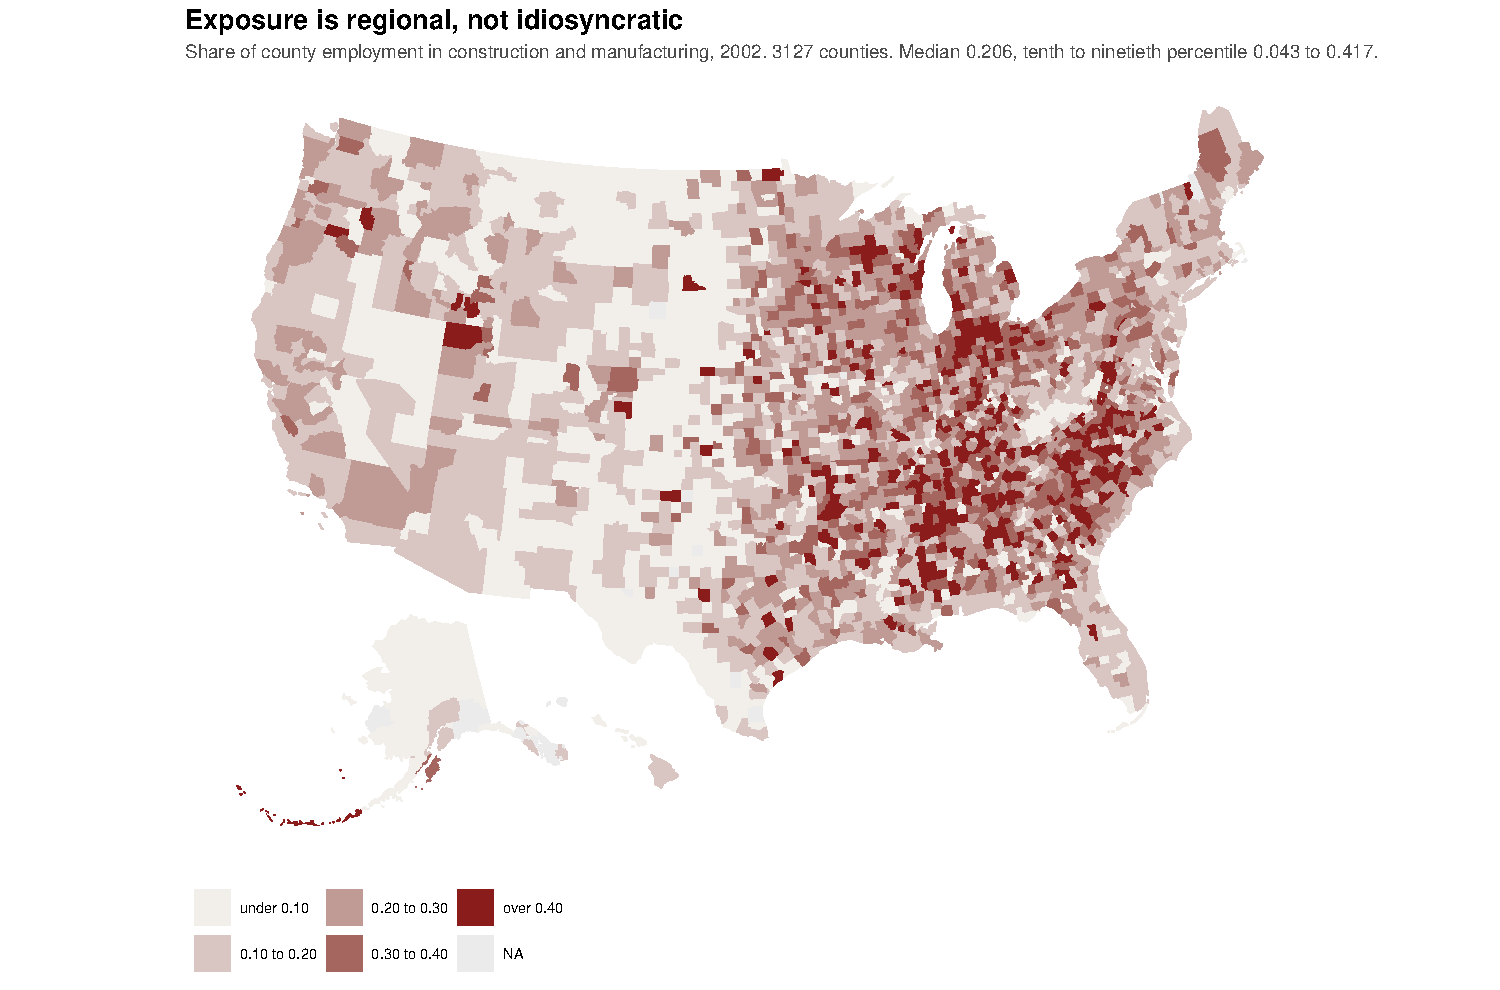
\includegraphics[width=\textwidth]{exposure_map_2002_rebuilt.pdf}
\caption{Exposure is regional, not idiosyncratic. Share of county employment in
construction and manufacturing, 2002, from County Business Patterns and held
fixed thereafter. 3{,}127 counties. Median $0.206$; tenth to ninetieth
percentile $0.043$ to $0.417$. Drawn on 2020 county boundaries: seven counties
whose FIPS codes were retired after 2002 have no polygon and are left blank.}
\label{fig:exposure}
\end{figure}

\begin{figure}[htbp]
\centering
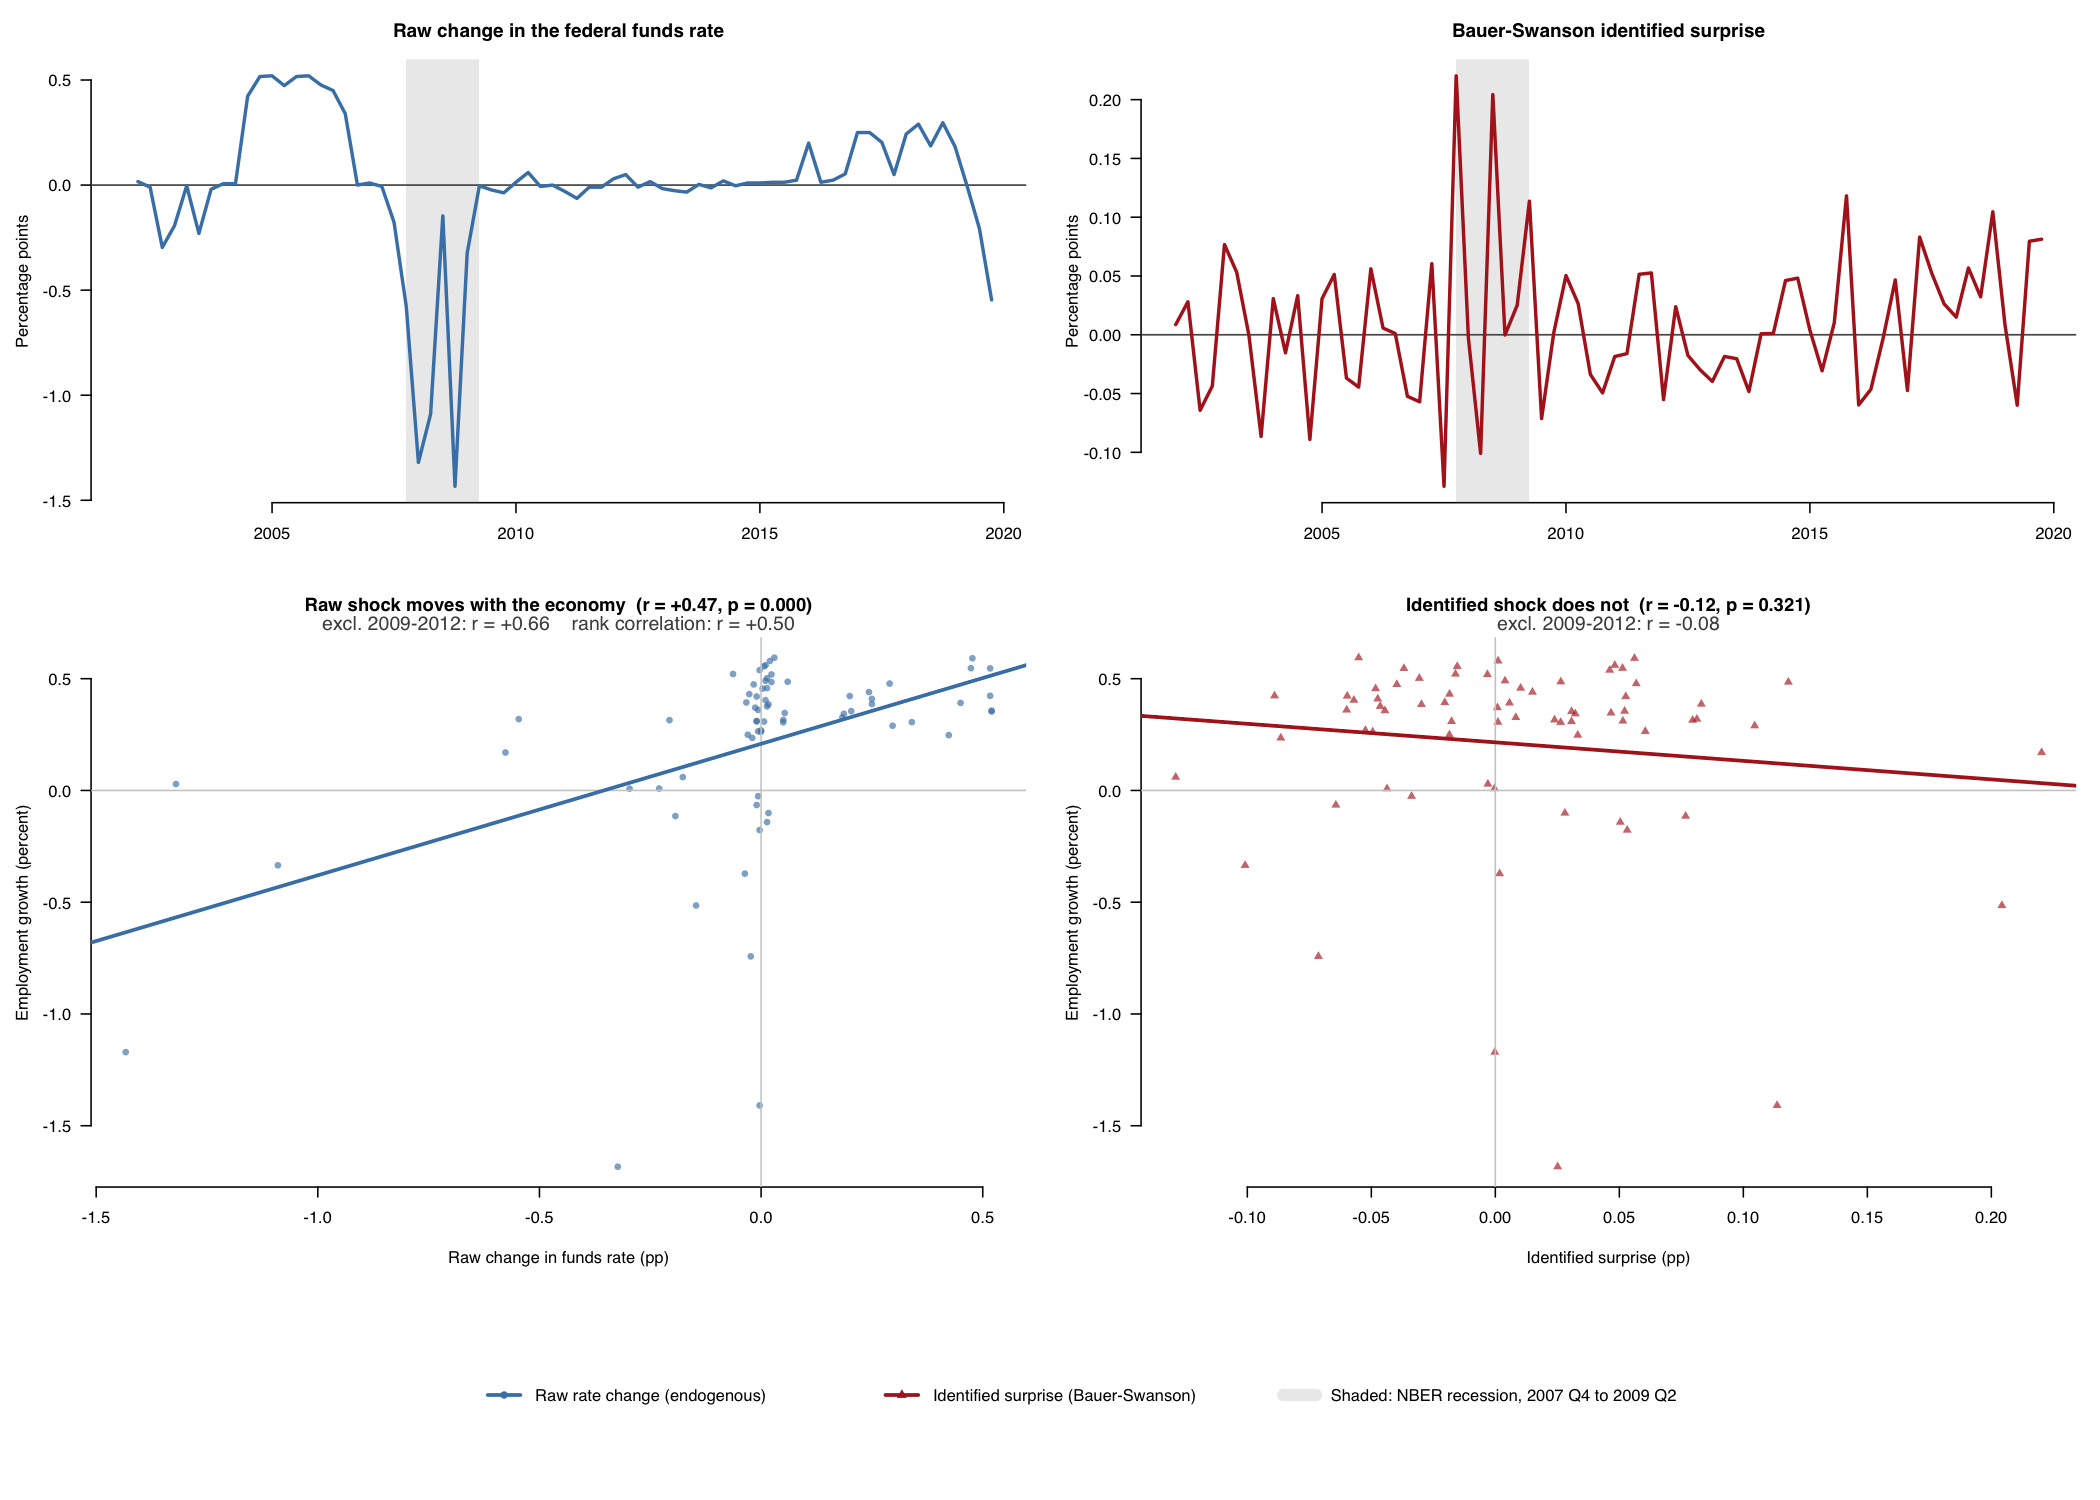
\includegraphics[width=\textwidth]{fig2_shock_comparison.png}
\caption{Two measures of monetary policy that share almost nothing. The realized
quarterly change in the federal funds rate against the orthogonalized
Bauer--Swanson high-frequency surprise, summed to quarters. Both series enter
the same design in the sections that follow; nothing else about the
specification changes between them.}
\label{fig:shocks}
\end{figure}

\begin{figure}[htbp]
\centering
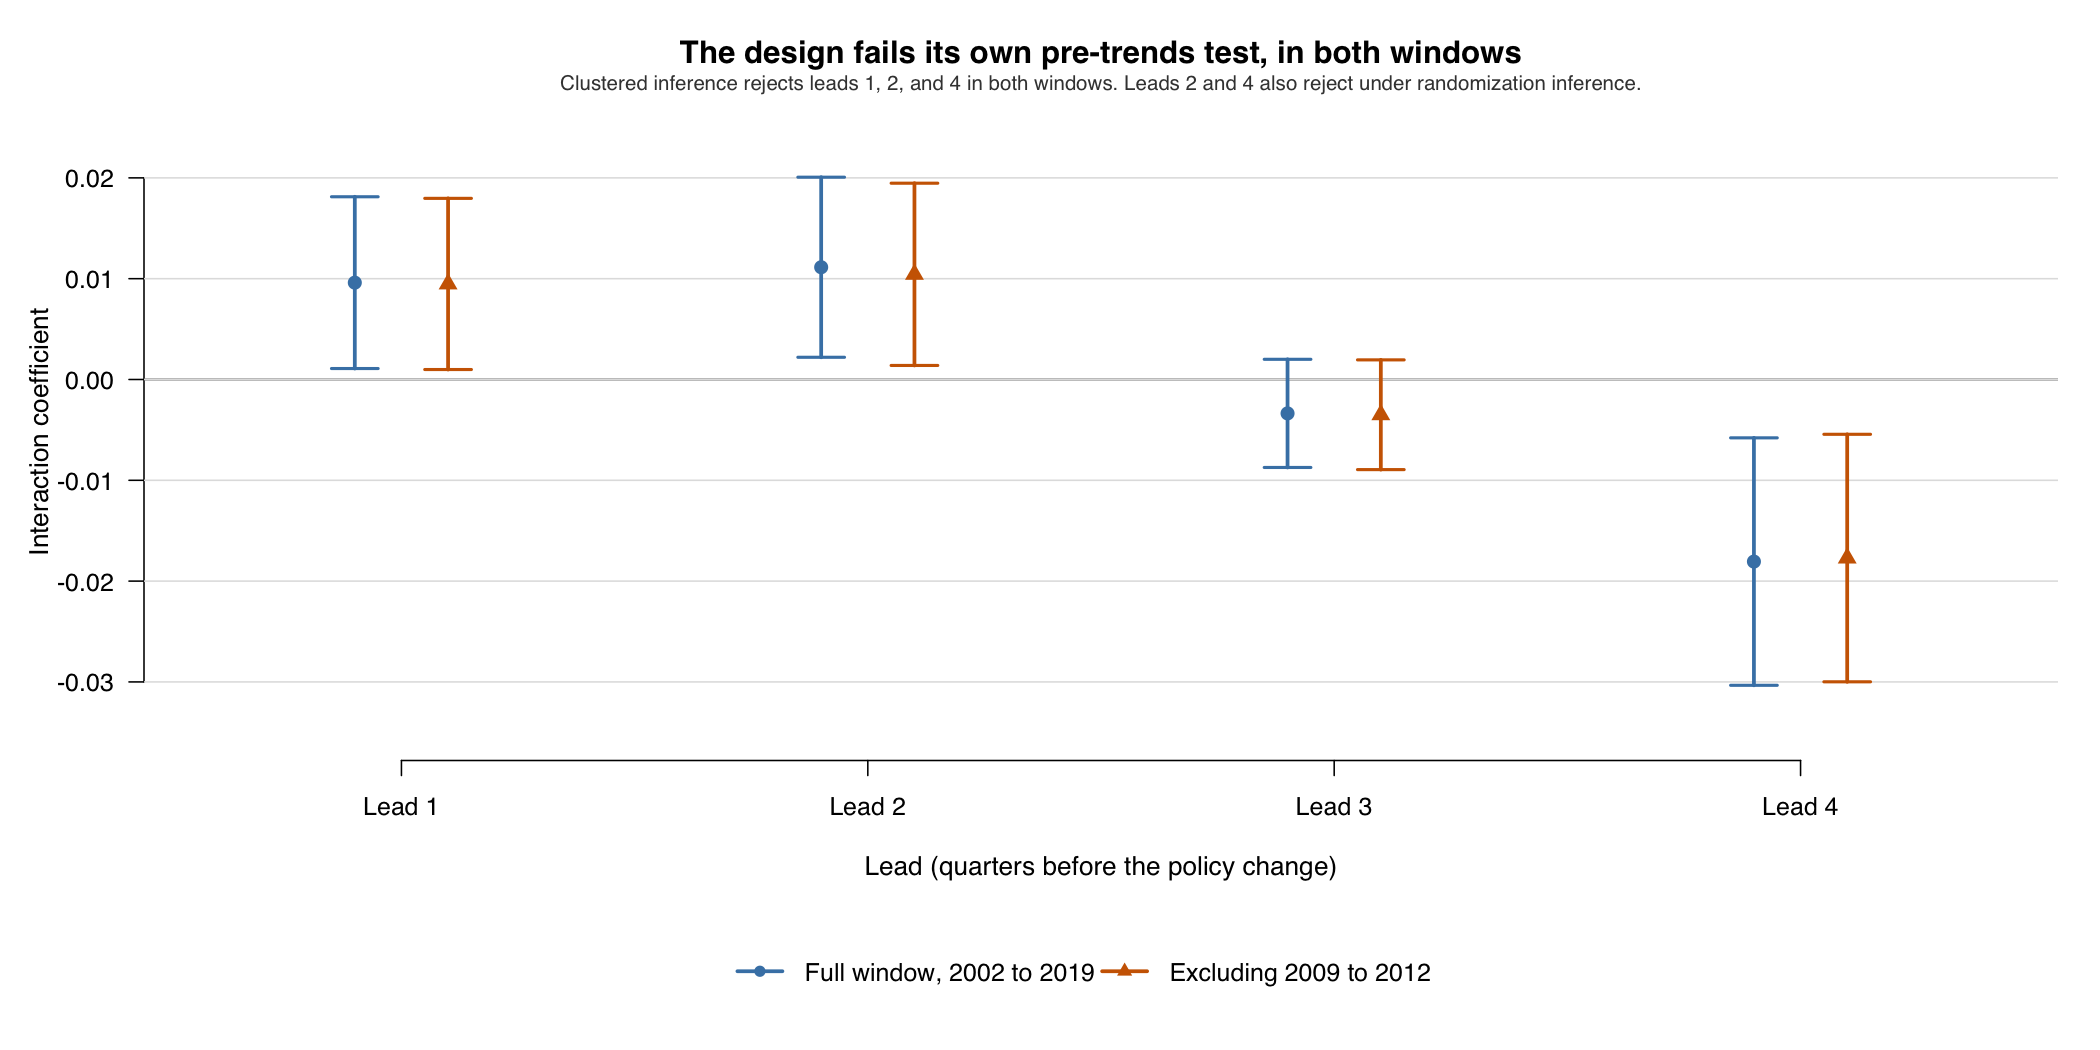
\includegraphics[width=\textwidth]{fig3_pretrends.png}
\caption{Pre-period leads of the exposure interaction, with 95 percent
confidence intervals, standard errors clustered by county. Leads are added to
the main specification; a design satisfying parallel trends would place all four
at zero. Estimates are shown for the full 2002 to 2019 panel and for the sample
excluding 2009 to 2012. Under clustered inference leads one, two and three
reject zero at five percent, and the two windows agree to within $0.0015$ on
every lead. The parallel-trends assumption fails regardless of the window, so
the difference-in-differences estimate cannot be read causally.}
\label{fig:pretrends}
\end{figure}

\begin{figure}[htbp]
\centering
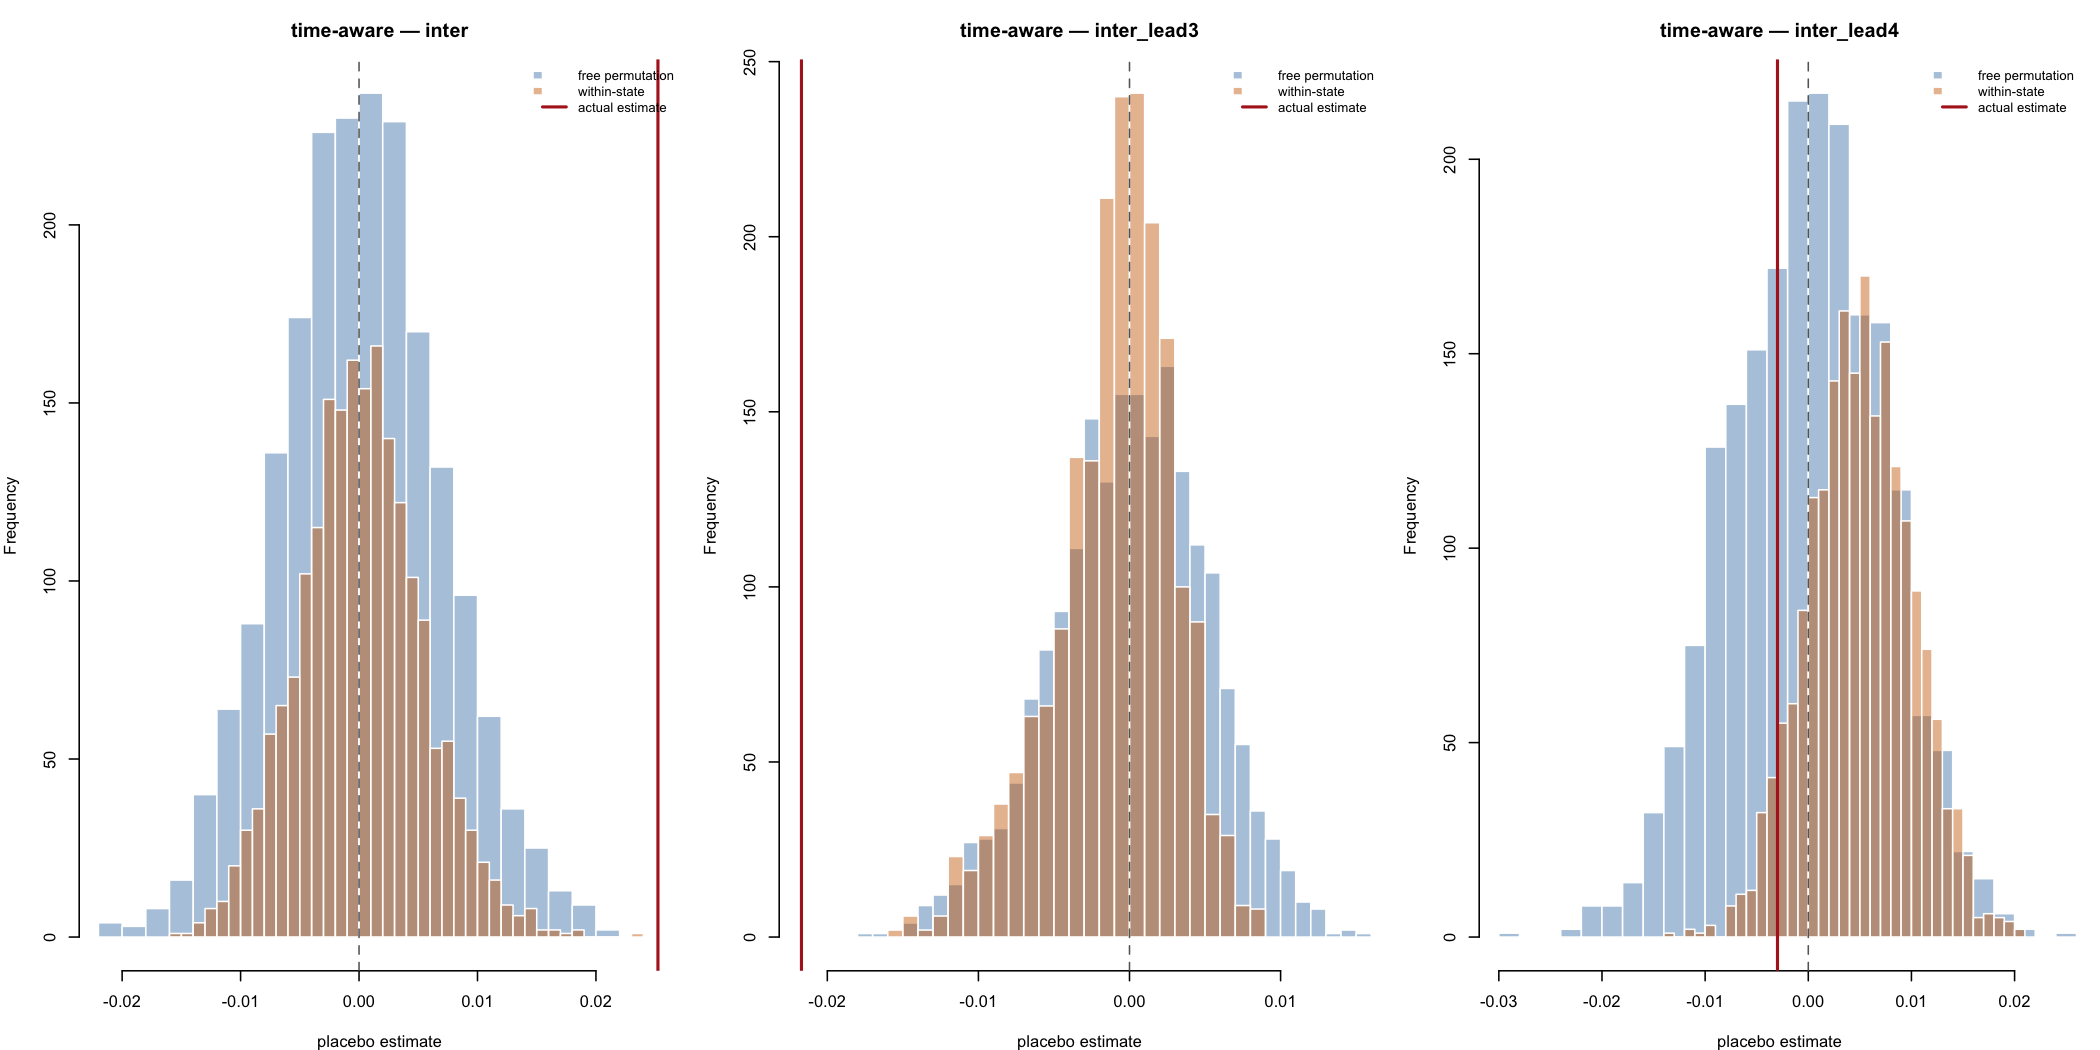
\includegraphics[width=\textwidth]{fig_randomization_inference_zlb-full.png}
\caption{Randomization inference on the pre-period leads. Exposure is permuted
across counties two thousand times and the model re-estimated on each draw; the
spread of the placebo estimates is the null distribution. The permutation spread
runs $1.11$ times the clustered standard error for the contemporaneous term and
$1.62$, $1.41$, $1.18$ and $0.76$ for the four leads, so the clustered errors are
too small for the first three leads. Leads two and three reject under
permutation, at $p=0.025$ and $p<0.0005$. Lead one is reported as unsettled:
$p=0.054$ against a Monte Carlo standard error of $0.005$.}
\label{fig:ri}
\end{figure}

% ⚠️ Figure 5 is fig4_raw_vs_identified.png. See the trap note at the top.
\begin{figure}[htbp]
\centering
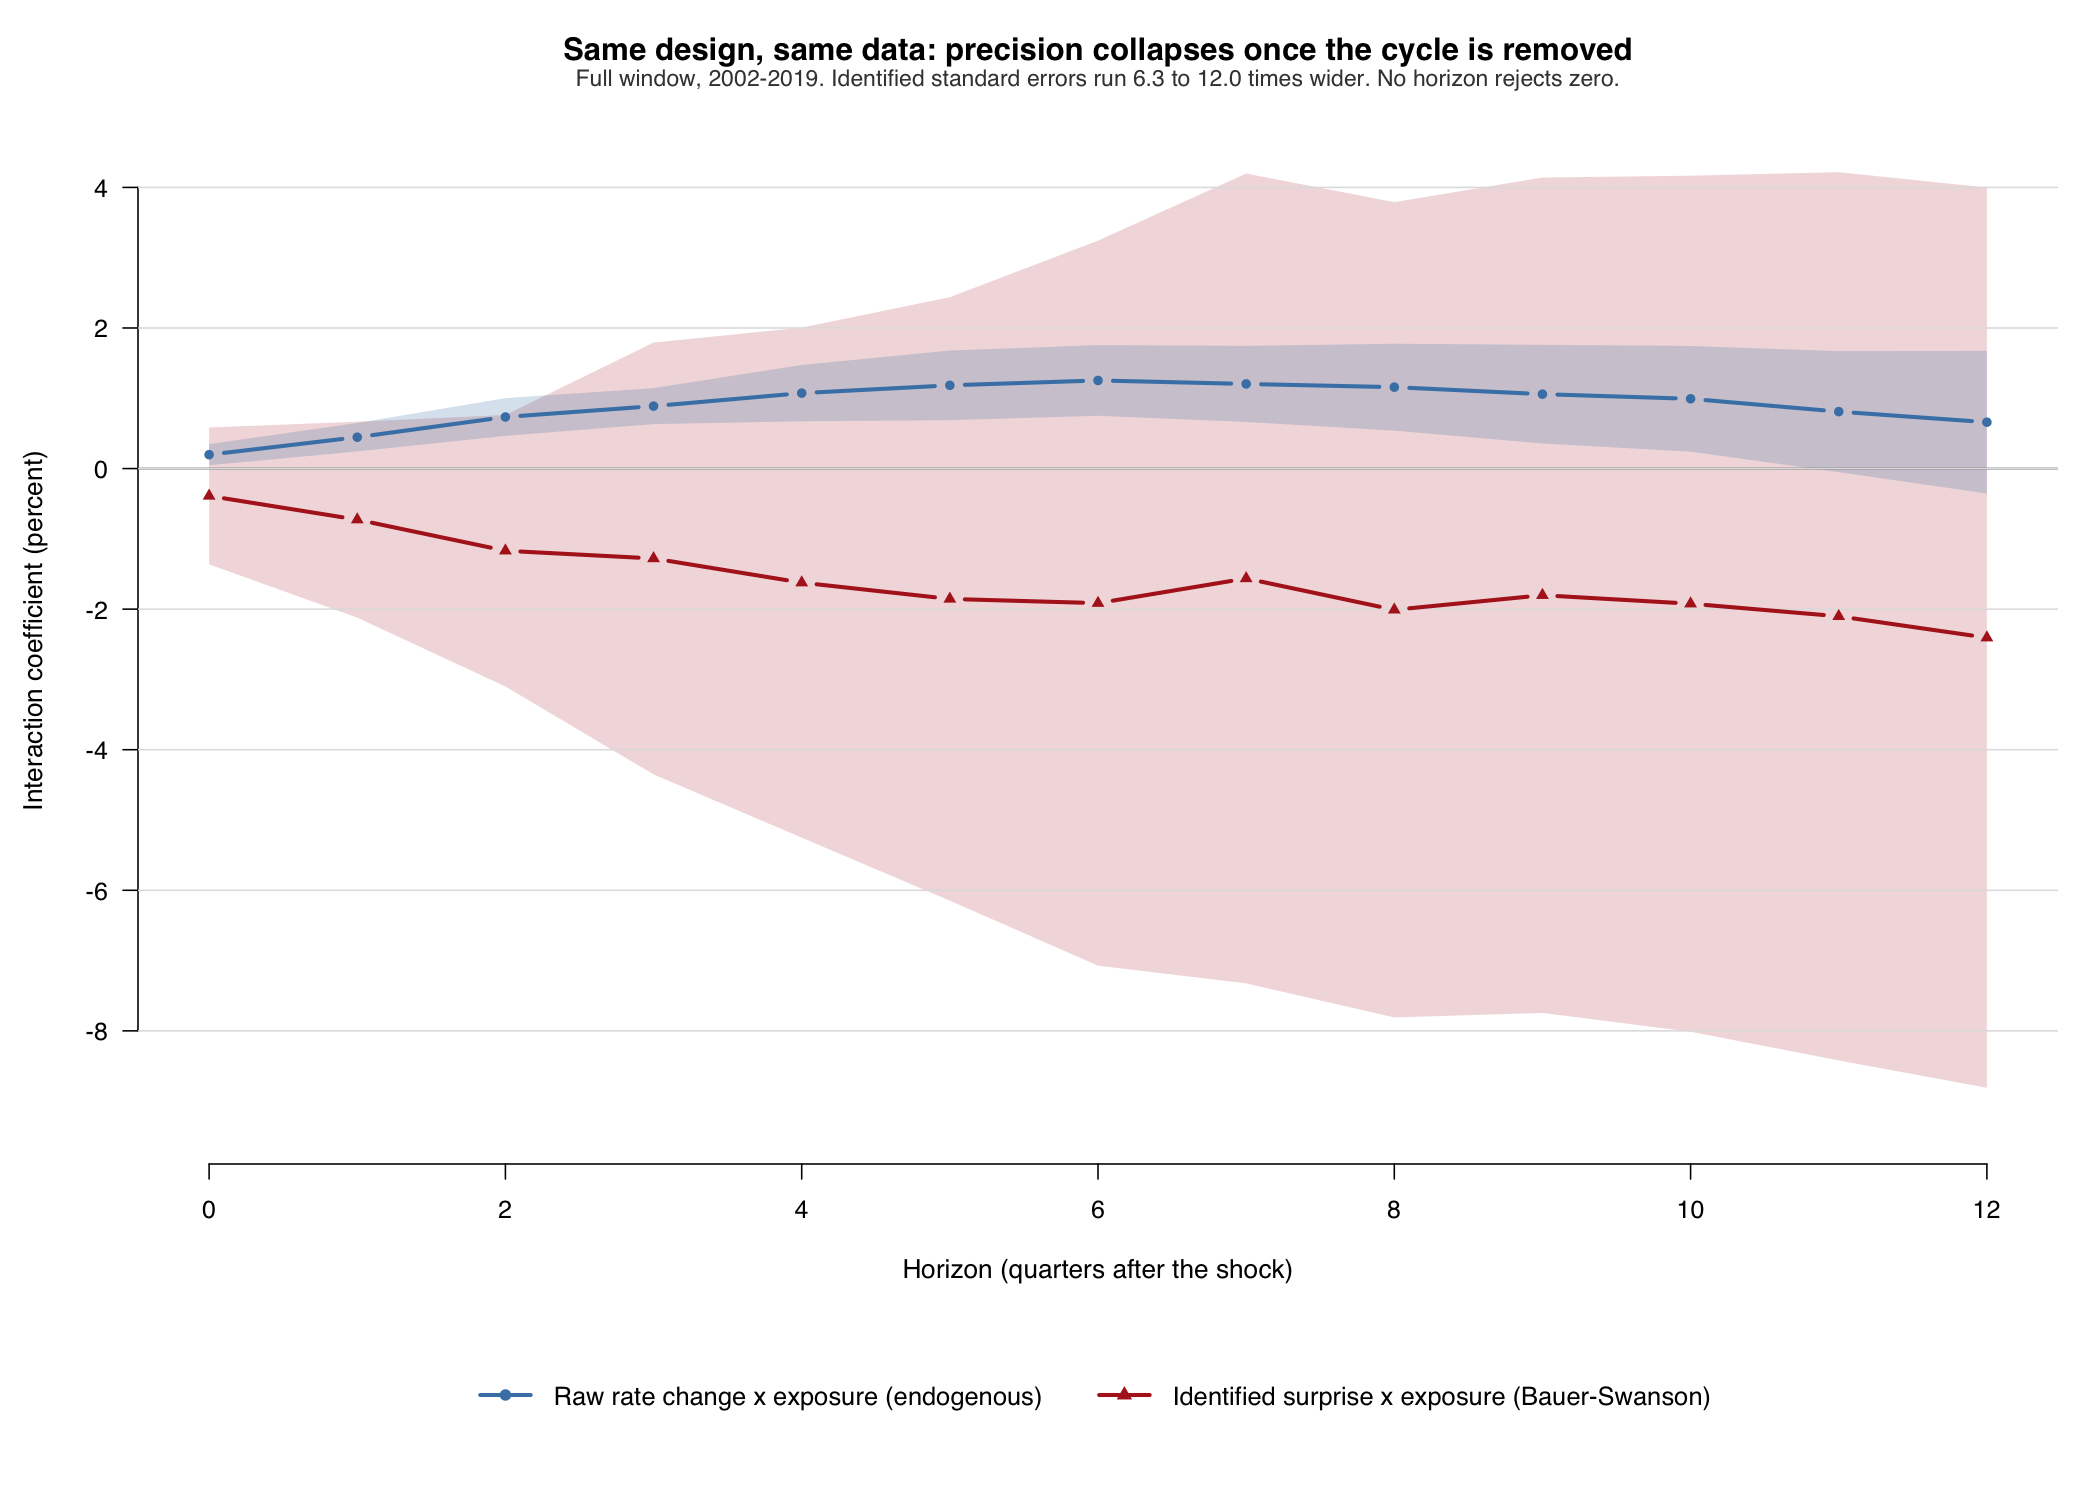
\includegraphics[width=\textwidth]{fig4_raw_vs_identified.png}
\caption{The same design, two shock measures. Local projections of the exposure
interaction across horizons zero to twelve, both sample windows. The raw
estimator uses the quarterly change in the federal funds rate; the identified
estimator substitutes Bauer--Swanson high-frequency surprises, holding the
design fixed. Raw estimates are positive at all thirteen horizons and
significant at eight; identified estimates are negative at all thirteen and
significant at none. The two estimators are not statistically distinguishable at
any horizon, the closest being $p=0.071$ at $h=2$, so the figure does not
establish a change in sign. It establishes a collapse in precision.}
\label{fig:lp}
\end{figure}

% ⚠️ Figure 6 is fig5_precision_collapse.png. See the trap note at the top.
\begin{figure}[htbp]
\centering
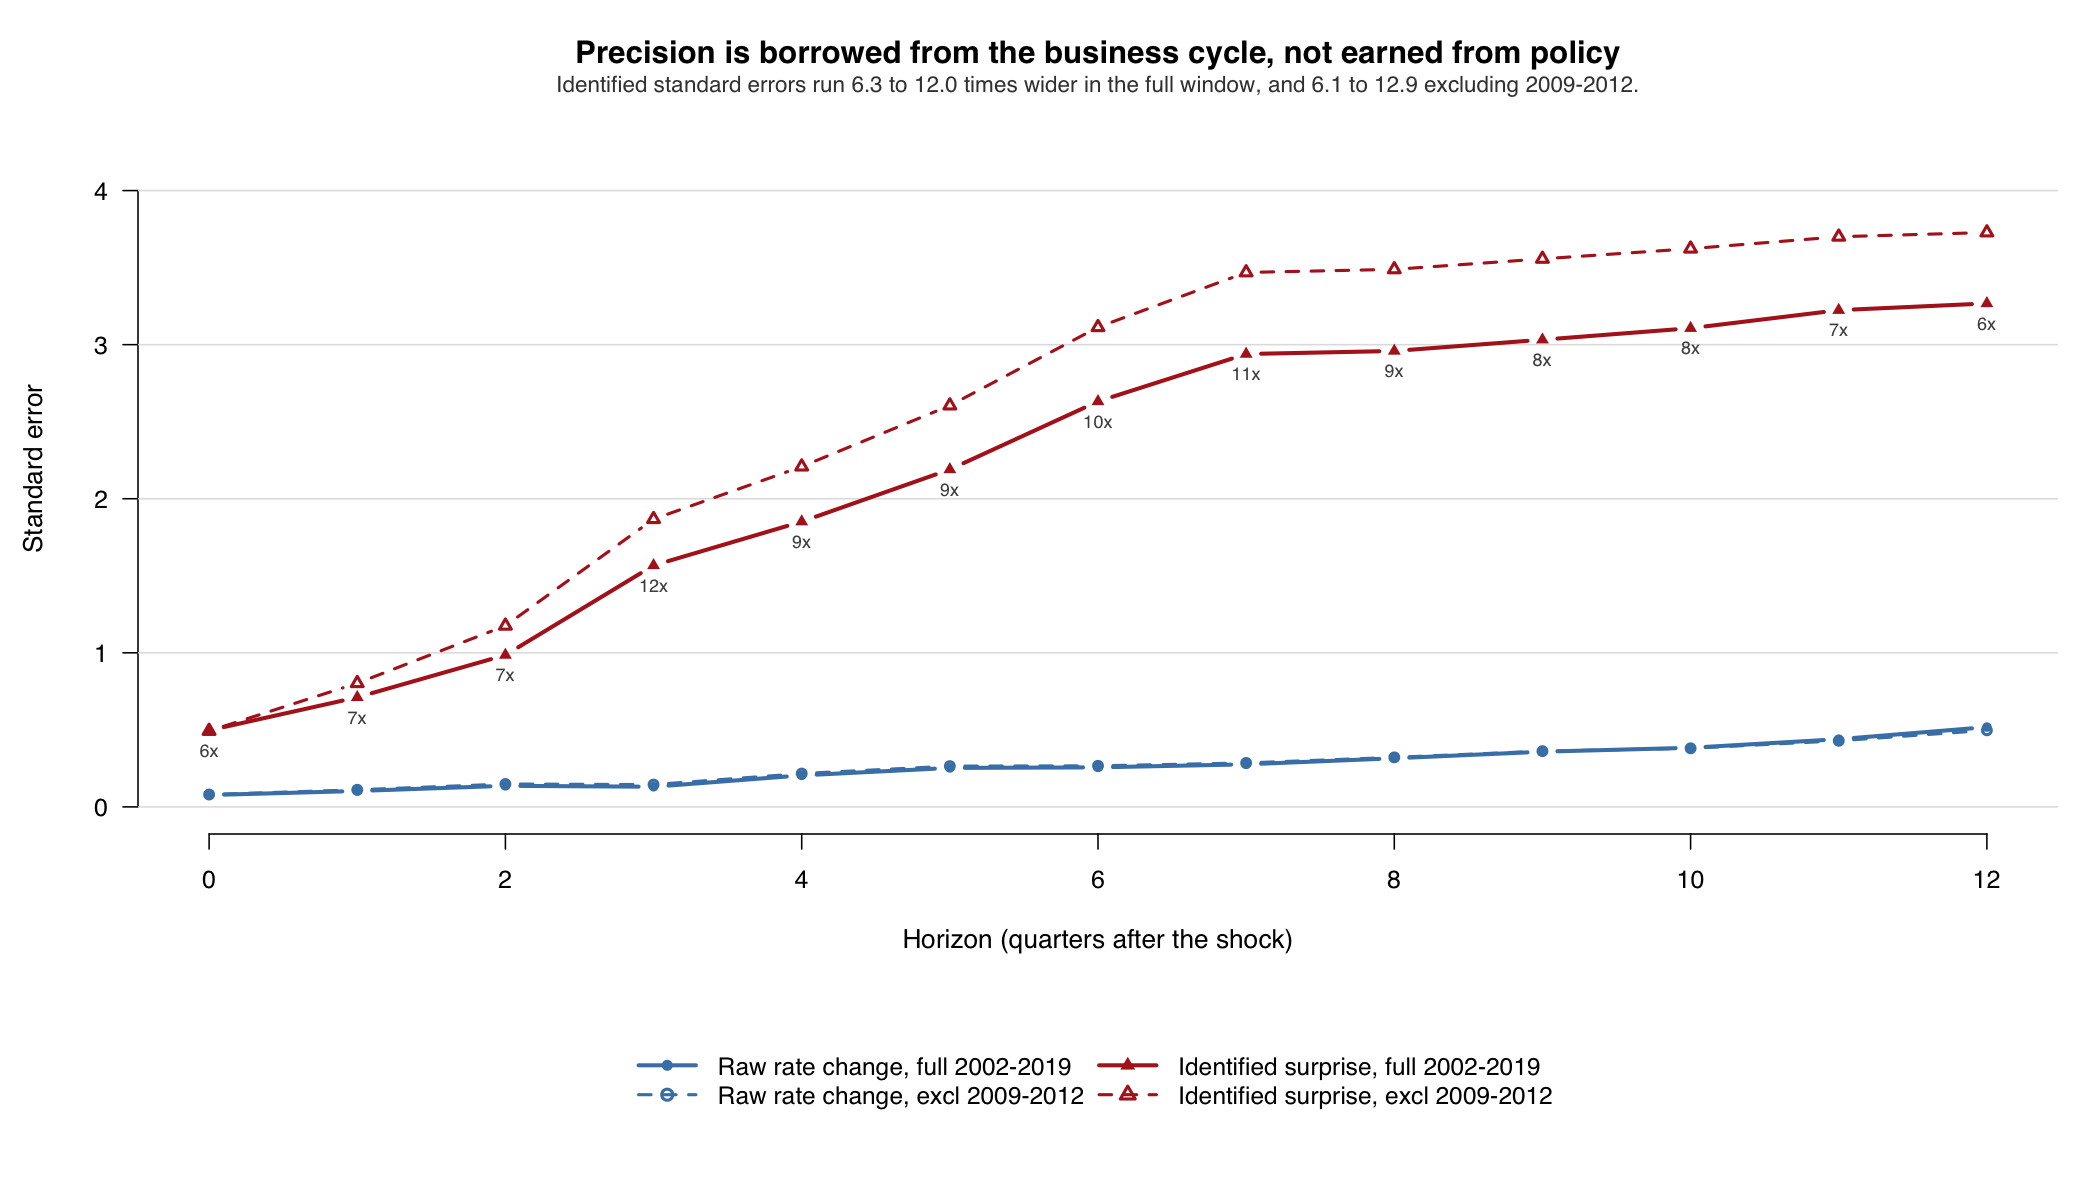
\includegraphics[width=\textwidth]{fig5_precision_collapse.png}
\caption{Precision, not sign, is what changes. Standard errors of the local
projection estimates by horizon, both sample windows. Colour distinguishes the
shock measure; line type distinguishes the window. Identified standard errors
run $5.3$ to $10.0$ times wider than raw ones over 2002--2019, and $5.8$ to
$11.7$ times wider excluding 2009--2012. The gap holds at every horizon in both
windows. Point estimates are in Figure~\ref{fig:lp}.}
\label{fig:precision}
\end{figure}

\clearpage
\begin{table}[htbp]
\centering
\caption{Shift-share difference-in-differences estimates of the exposure interaction. The outcome is log county employment. Exposure is the 2002 County Business Patterns share of county employment in construction and manufacturing, held fixed. Standard errors, clustered by county, in parentheses. 3,127 counties. $^{***}p<0.01$, $^{**}p<0.05$, $^{*}p<0.10$.}
\label{tab:main}
\begin{tabular}{lcc}
\toprule
 & Full panel & Excluding \\
 & 2002--2019 & 2009--2012 \\
 & (1) & (2) \\
\midrule
Exposure $\times\ \Delta$ federal funds rate & 0.0332$^{***}$ & 0.0318$^{***}$ \\
 & (0.0066) & (0.0064) \\
\midrule
County fixed effects & Yes & Yes \\
Quarter fixed effects & Yes & Yes \\
Observations & 224,952 & 174,968 \\
\bottomrule
\end{tabular}

\begin{minipage}{0.92\textwidth}\vspace{4pt}\footnotesize The two estimates differ by $0.0014$, about a fifth of a standard error, so the result is not produced by the zero-lower-bound period. Section~\ref{sec:lp} shows that this precision does not survive an identified shock.\end{minipage}
\end{table}


\begin{table}[htbp]
\centering
\caption{Pre-trends test. Four leads of the exposure interaction are added to the main specification. Under parallel trends all four are zero. Standard errors, clustered by county, in parentheses. $^{***}p<0.01$, $^{**}p<0.05$, $^{*}p<0.10$.}
\label{tab:placebo}
\begin{tabular}{lcc}
\toprule
 & Full panel & Excluding \\
 & 2002--2019 & 2009--2012 \\
 & (1) & (2) \\
\midrule
Exposure $\times\ \Delta$ federal funds rate & 0.0252$^{***}$ & 0.0229$^{***}$ \\
 & (0.0060) & (0.0057) \\
\quad lead 1 & 0.0157$^{***}$ & 0.0146$^{***}$ \\
 & (0.0052) & (0.0052) \\
\quad lead 2 & 0.0172$^{***}$ & 0.0157$^{***}$ \\
 & (0.0055) & (0.0055) \\
\quad lead 3 & -0.0217$^{***}$ & -0.0226$^{***}$ \\
 & (0.0043) & (0.0044) \\
\quad lead 4 & -0.0030 & -0.0019 \\
 & (0.0097) & (0.0098) \\
\midrule
County fixed effects & Yes & Yes \\
Quarter fixed effects & Yes & Yes \\
Observations & 212,468 & 162,484 \\
\bottomrule
\end{tabular}

\begin{minipage}{0.92\textwidth}\vspace{4pt}\footnotesize Leads one, two and three reject zero at five percent in both windows, so the parallel-trends assumption fails and the difference-in-differences estimate cannot be read causally. The paper reports a count of two, the leads that also reject under randomization inference; see Section~\ref{sec:pretrends}.\end{minipage}
\end{table}



% =============================================================================
\clearpage
\bibliographystyle{aer}
\bibliography{references}

\end{document}
